In this section, we focus on instantaneous spanwise vorticity for the different meshes considered due to zonal-based refinement/adaptation. 
Instantaneous data is considered here since we are interested in observing the flow structures and turbulence captured by different meshes, and obtaining phase-averaged data over multiple cycles can be computationally expensive, especially for the finer meshes, and can also filter out the turbulence in the flow-field.

A comparison of instantaneous spanwise vorticity for the different meshes is shown in Figures \ref{fig:vorticity_zonal_150}, \ref{fig:vorticity_zonal_180}, \ref{fig:vorticity_zonal_210}, \ref{fig:vorticity_zonal_240}, and \ref{fig:vorticity_zonal_270} for phases $\psi=150^\circ$, $\psi=180^\circ$, $\psi=210^\circ$, $\psi=240^\circ$, and $\psi=270^\circ$ respectively. 

For $\psi=150^\circ$, as the airfoil decelerates, the boundary layer over the airfoil starts to roll-up towards the geometric leading edge. The finer meshes, Mza2 and Mza3, show a thicker boundary layer along with more resolution of turbulence/fine-scale structures than
the coarser meshes, M0 and Mza1.

For $\psi=180^\circ$, Mza2 and Mza3 meshes show a thicker boundary layer roll-up towards the geometric leading edge over the airfoil surface, as compared to $\psi=150^\circ$, along with flow separation. 
M0 and Mza1 meshes fail to capture a significant boundary layer roll-up at this phase. 
Moreover, Mza2 and Mza3 meshes capture more turbulence than M0 and Mza1 meshes, with the flow-structures captured by Mza2 meshes being slightly more diffused than Mza3 meshes. 
Note that changes in spanwise resolution considered here for the same in-plane mesh do not show any significant variations in the flow-field.

For $\psi=210^\circ$, formation of LEV begins to take place for all meshes apart from M0, as we see a distinct vortex build up near the geometric leading edge, which M0 mesh fails to capture. 
There is a clear difference between both the location of the roll-up over the airfoil surface, and the size and extent of the roll-up between Mza1 meshes and Mza2 and Mza3 meshes.
The flow-field for Mza2 and Mza3 meshes compare well with each other, with some minor differences.
More fine-scale flow structures are resolved by the finer meshes Mza2 and Mza3, while M0 and Mza1 show poor resolution of these structures.

At $\psi=240^\circ$, the LEV has ejected from the airfoil surface into a distinct vortex. 
Once again, a clear difference can be observed between the coarser meshes (M0 and Mza1 meshes) and the finer meshes (Mza2 and Mza3 meshes), in position, size, and extent of the LEV core, and also the turbulence captured around the LEV core. 
The coarsest mesh, M0, shows very poor resolution of the shear layer, LEV, and the fine scale structures around it. 
Mza1 meshes also show poor resolution of shear layer of LEV core and flow structures around it as compared to the finer meshes, along with significant difference in the location, size, and extent of LEV core.
Mza2 and Mza3 meshes compare well with each other in terms of the shear layer, LEV location, size, and extent, as well as the fine scale structures resolved.
Once again, note that changes in spanwise resolution for the same in-plane mesh do not show any significant variations in the flow-field. 

At $\psi=270^\circ$, M0 mesh shows poor resolution with a diffused LEV core as compared to the other meshes, along with poor resolution of the shear layer.
Mza1 meshes show a less diffused LEV core as compared to M0 mesh, however, the shear layer has comparatively poor resolution when compared to the finer meshes Mza2 and Mza3. 
Mza1 meshes also show minimal fine scale structures around the LEV core, as compared to Mza2 and Mza3 meshes. 
The LEV and the shear layer are best resolved in Mza3 meshes, with Mza3 showing more fine scale structures around the LEV core than Mza2 meshes.

A more quantitive comparison of the LEV including tangential velocity profiles and LEV location for different phases in the surging cycle is mentioned in the following sections.

%%=====================================
%% Phase = 150
%%=====================================


\begin{figure}[H]
	\centering
	\begin{center}
		\begin{subfigure}[b]{0.475\textwidth}
			\centering
			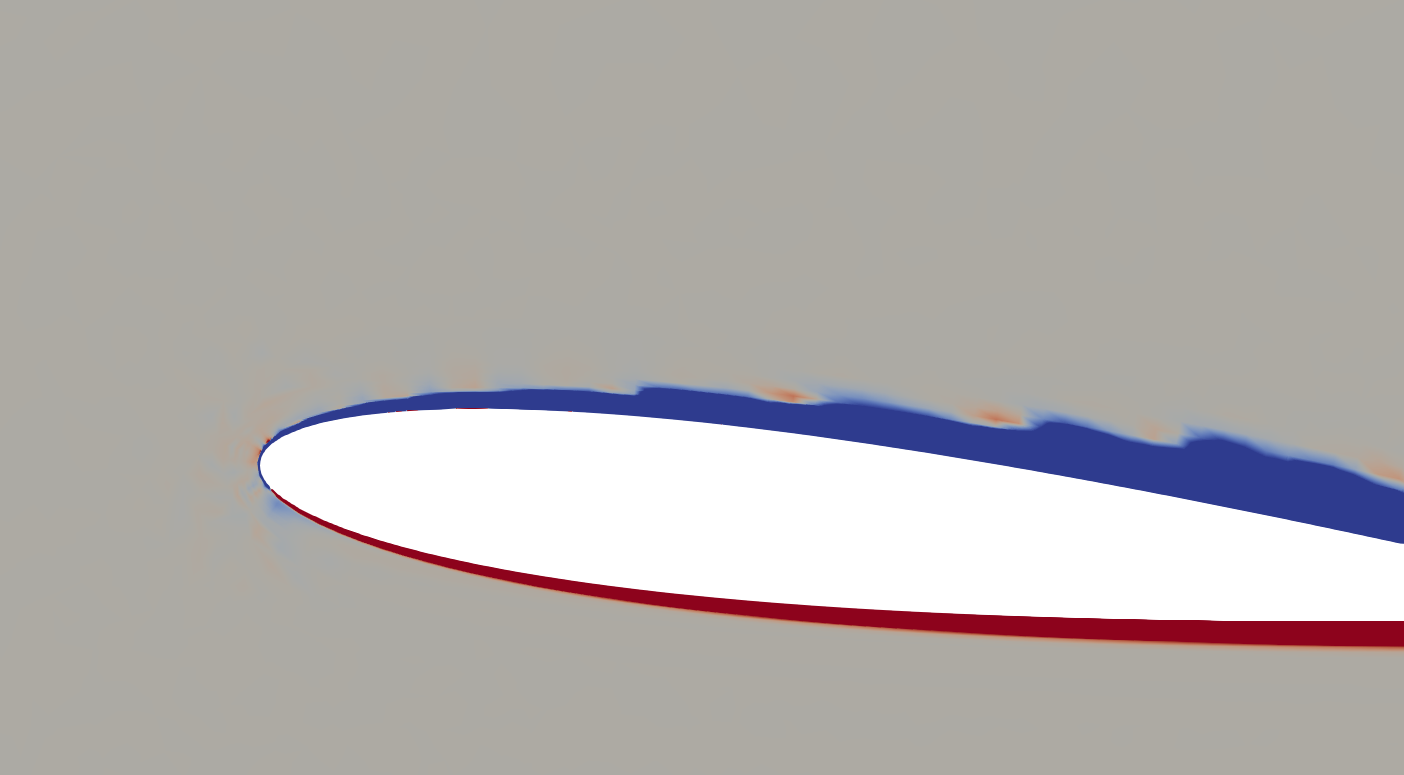
\includegraphics[width=1\textwidth]{figures/zonal_adapt_results/vorticity_plots/v2/M0/spavg/phase_150.png}
			\caption{M0\_nz25 mesh, $\psi$ = $150^\circ$}
			\label{fig:M0_sp_psi150}
		\end{subfigure}
	\end{center}
	\begin{subfigure}[b]{0.475\textwidth}
		\centering
		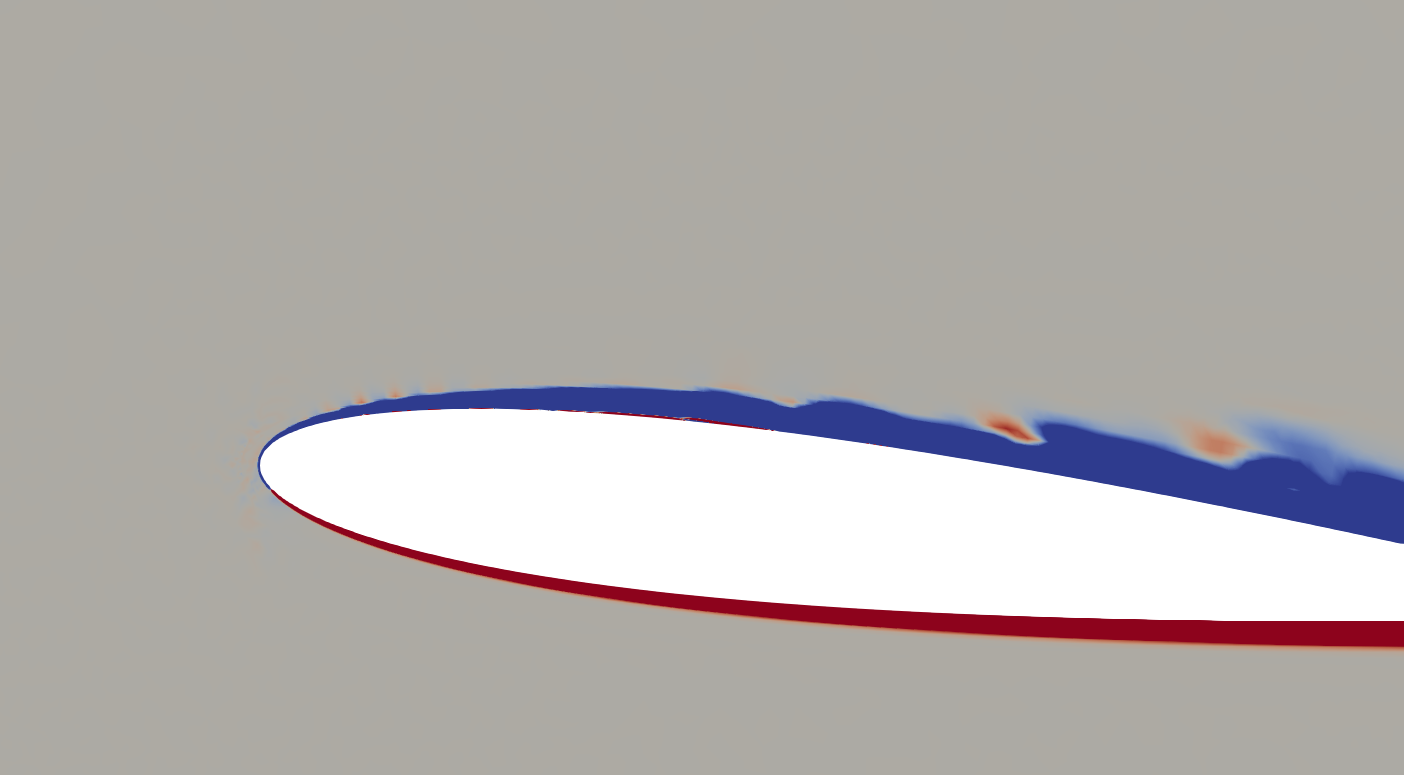
\includegraphics[width=1\textwidth]{figures/zonal_adapt_results/vorticity_plots/v2/Mza1_25/spavg/phase_150.png}
		\caption{Mza1\_nz25 mesh, $\psi$ = $150^\circ$}
		\label{fig:Mza1_25_sp_psi150}
	\end{subfigure}
	\begin{subfigure}[b]{0.475\textwidth}
		\centering
		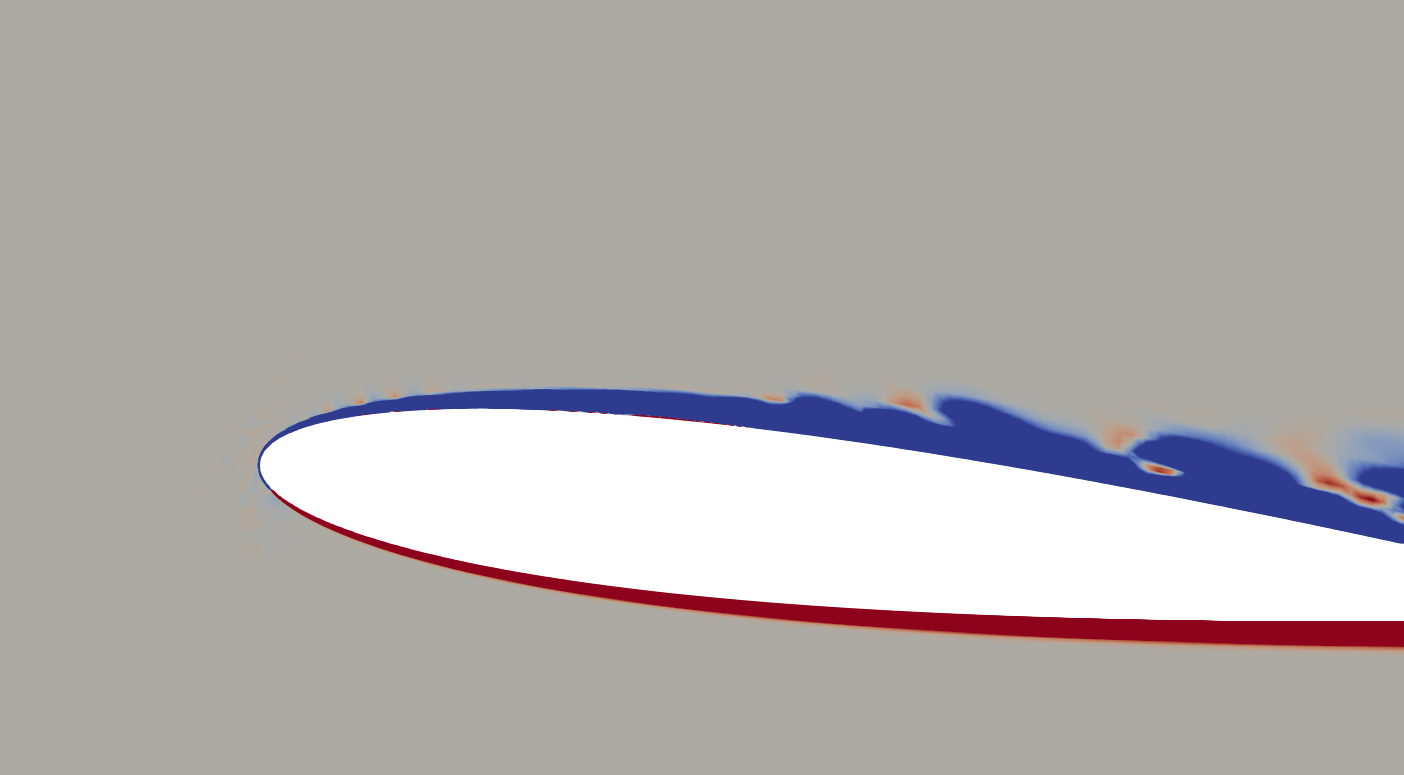
\includegraphics[width=1\textwidth]{figures/zonal_adapt_results/vorticity_plots/v2/Mza1_50/spavg/phase_150.png}
		\caption{Mza1\_nz50 mesh, $\psi$ = $150^\circ$}
		\label{fig:Mza1_50_sp_psi150}
	\end{subfigure}
	%	\begin{subfigure}[b]{0.475\textwidth}
	%		\centering
	%		\includegraphics[width=1\textwidth]{figures/zonal_adapt_results/vorticity_plots/v2/Mza1_100/spavg/phase_150.png}
	%		\caption{Mza1\_100 mesh, $\psi$ = $150^\circ$}
	%		\label{fig:Mza1_100_sp_psi150}
	%	\end{subfigure}
	%	\begin{subfigure}[b]{0.475\textwidth}
	%	\centering
	%	\includegraphics[width=1\textwidth]{figures/zonal_adapt_results/vorticity_plots/v2/Mza2_25/spavg/phase_150.png}
	%	\caption{Mza2\_25 mesh, $\psi$ = $150^\circ$}
	%	\label{fig:Mza2_25_sp_psi150}
	%	\end{subfigure}
	\begin{subfigure}[b]{0.475\textwidth}
		\centering
		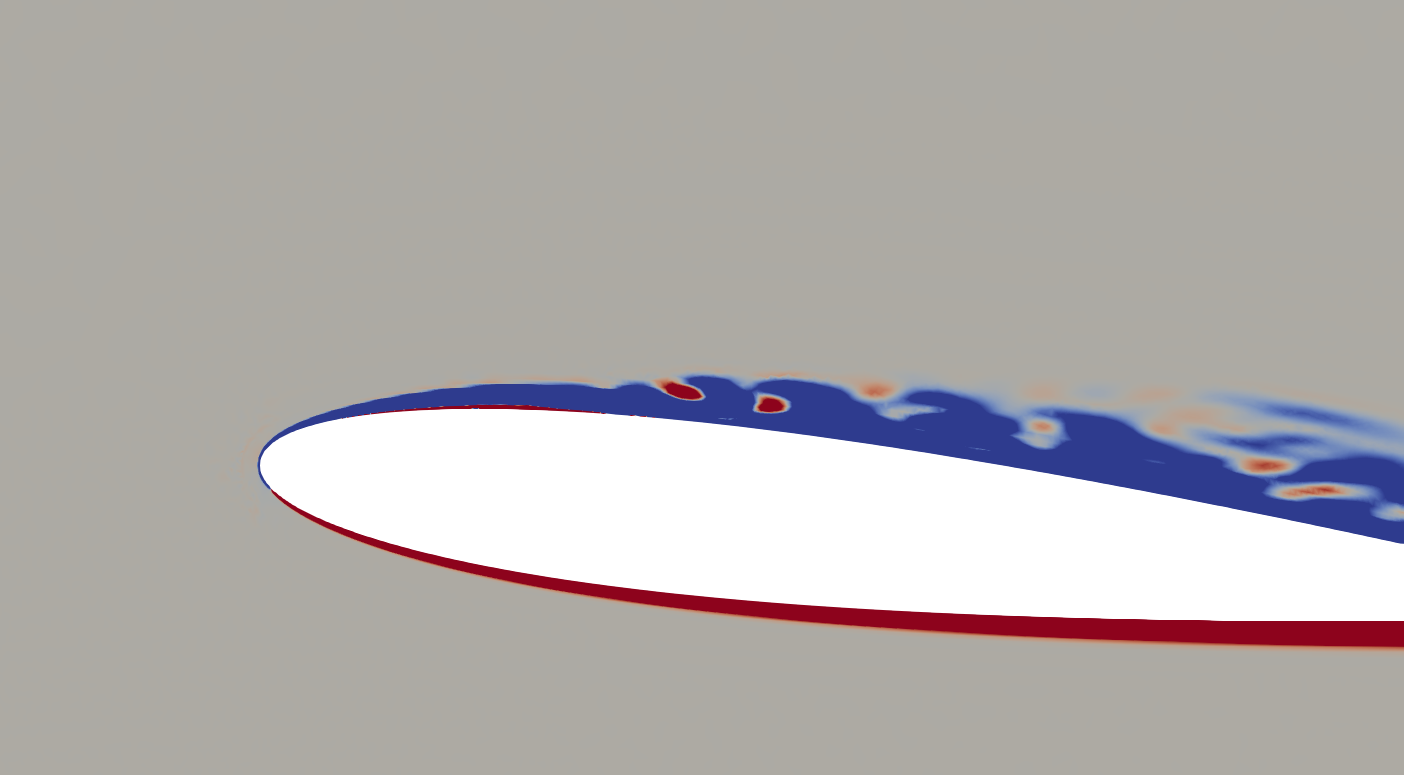
\includegraphics[width=1\textwidth]{figures/zonal_adapt_results/vorticity_plots/v2/Mza2_50/spavg/phase_150.png}
		\caption{Mza2\_nz50 mesh, $\psi$ = $150^\circ$}
		\label{fig:Mza2_50_sp_psi150}
	\end{subfigure}	
	\begin{subfigure}[b]{0.475\textwidth}
		\centering
		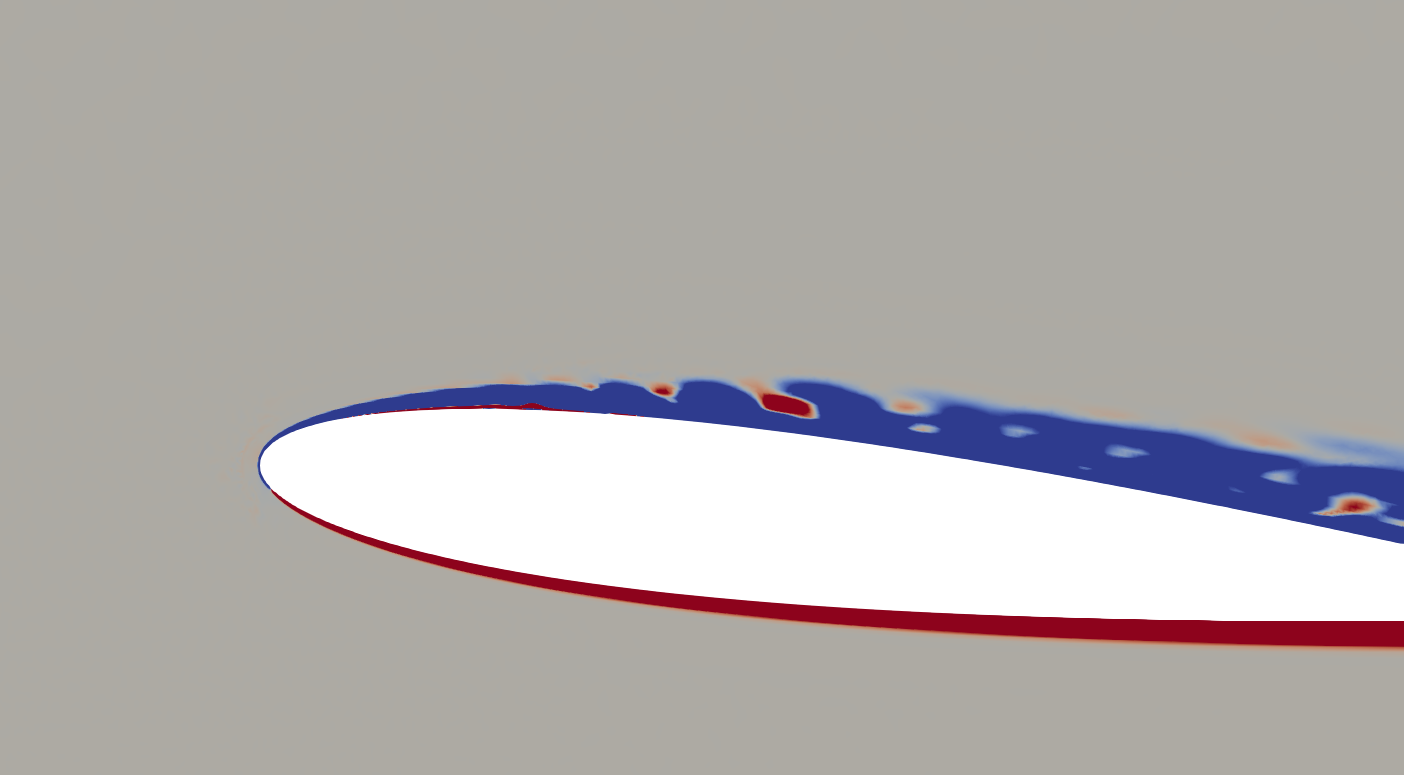
\includegraphics[width=1\textwidth]{figures/zonal_adapt_results/vorticity_plots/v2/Mza2_100/spavg/phase_150.png}
		\caption{Mza2\_nz100 mesh, $\psi$ = $150^\circ$}
		\label{fig:Mza2_100_sp_psi150}
	\end{subfigure}
	\begin{subfigure}[b]{0.475\textwidth}
		\centering
		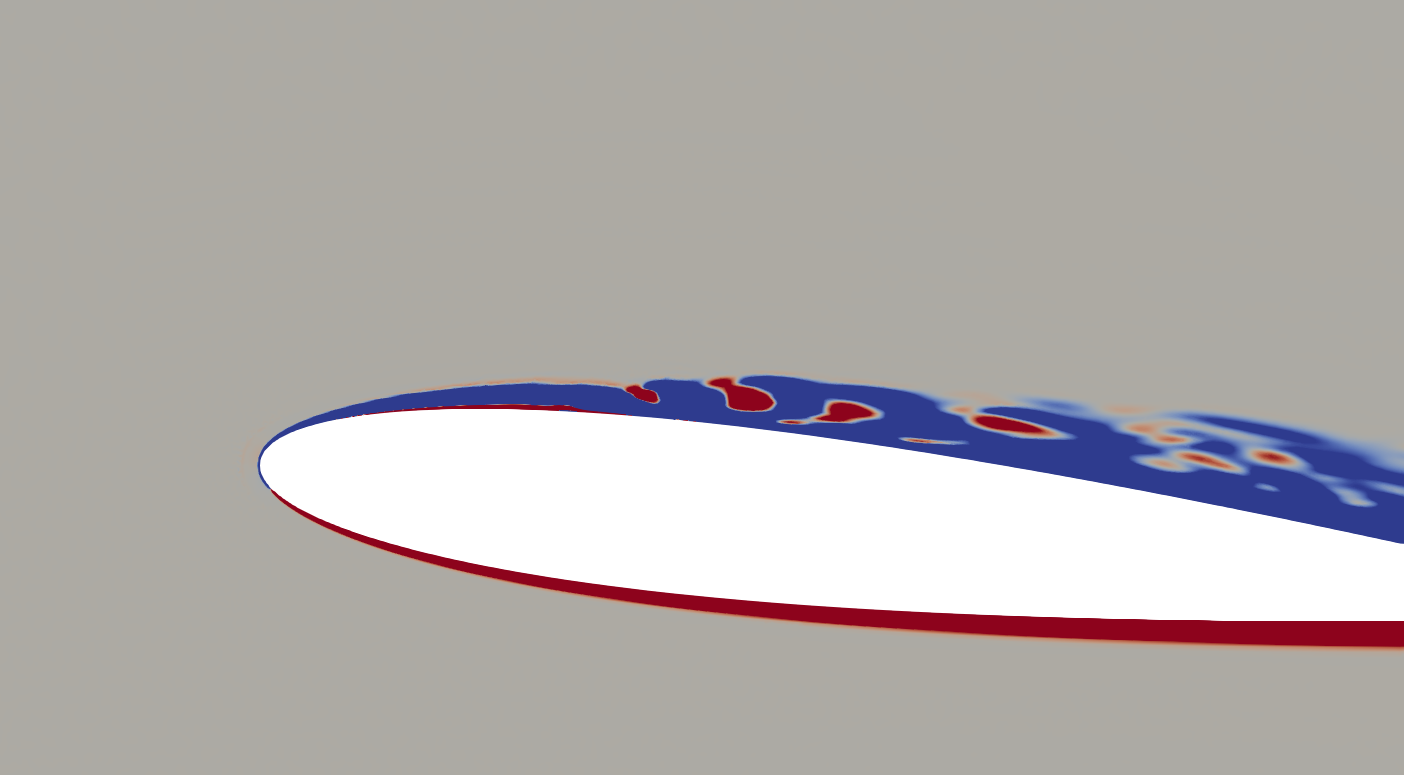
\includegraphics[width=1\textwidth]{figures/zonal_adapt_results/vorticity_plots/v2/Mza3_50/spavg/phase_150.png}
		\caption{Mza3\_nz50 mesh, $\psi$ = $150^\circ$}
		\label{fig:Mza3_50_sp_psi150}
	\end{subfigure}
	\begin{subfigure}[b]{0.475\textwidth}
		\centering
		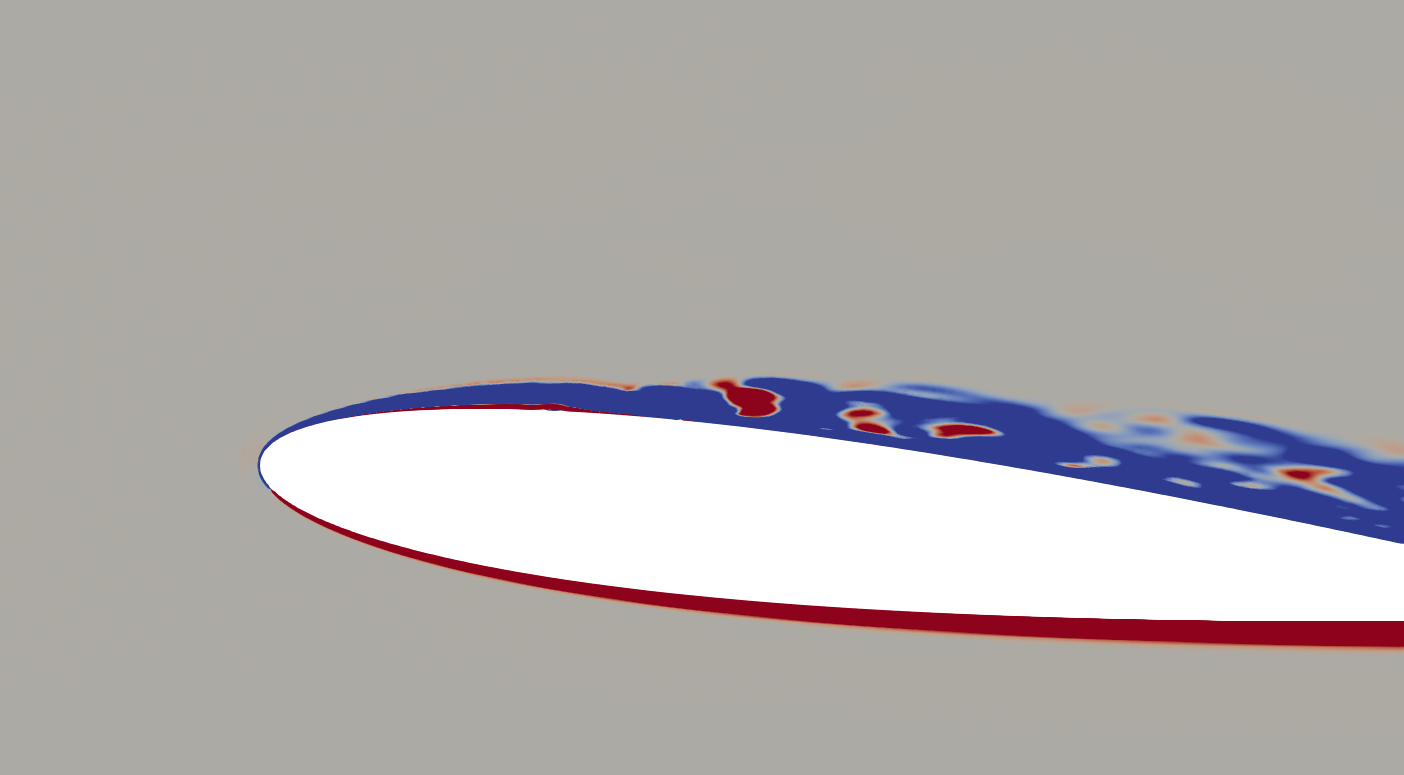
\includegraphics[width=1\textwidth]{figures/zonal_adapt_results/vorticity_plots/v2/Mza3_100/spavg/phase_150.png}
		\caption{Mza3\_nz100 mesh, $\psi$ = $150^\circ$}
		\label{fig:Mza3_100_sp_psi150}
	\end{subfigure}
	\caption{Spanwise vorticity comparison at $\psi$ = $150^\circ$ for different meshes}
	\label{fig:vorticity_zonal_150}
\end{figure}




%%=====================================
%% Phase = 180
%%=====================================


\begin{figure}[H]
	\centering
	\begin{center}
	\begin{subfigure}[b]{0.475\textwidth}
		\centering
		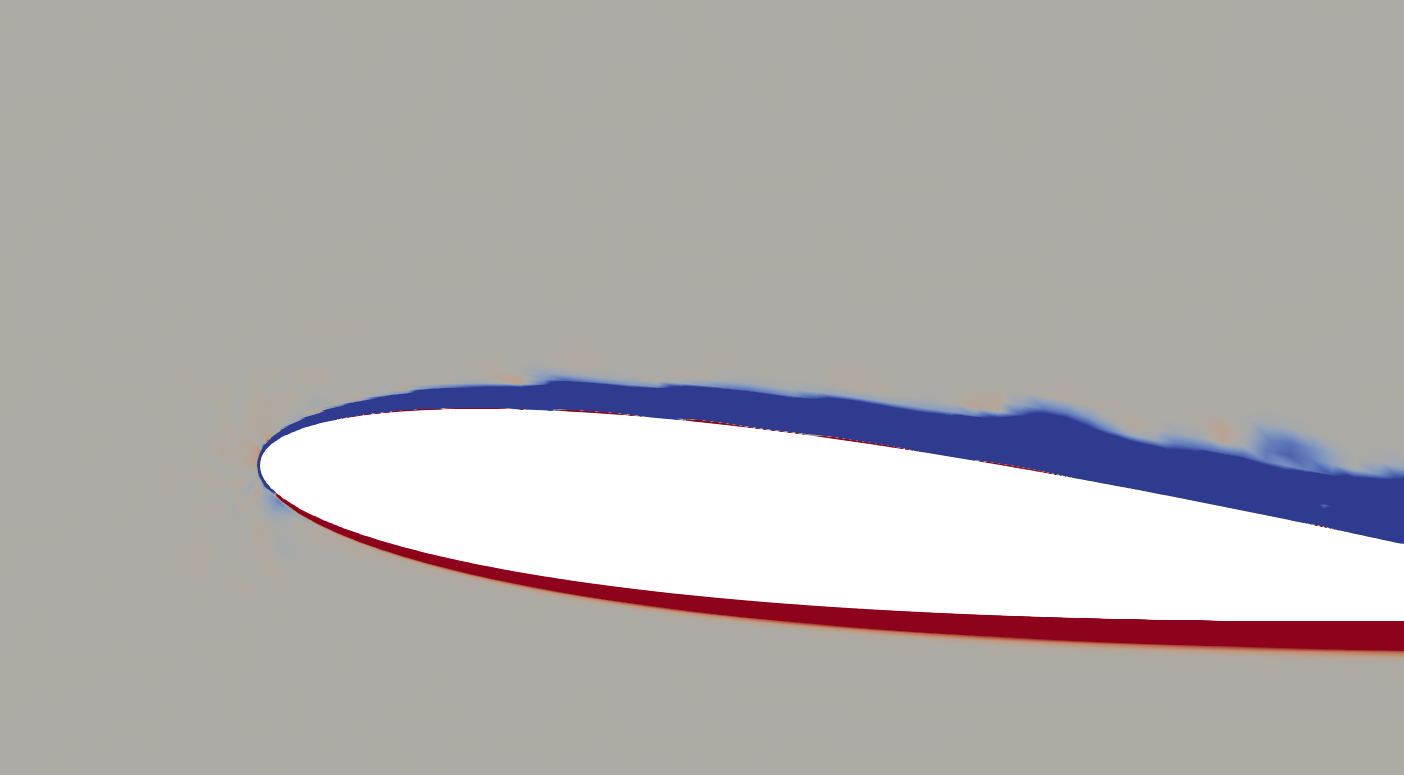
\includegraphics[width=1\textwidth]{figures/zonal_adapt_results/vorticity_plots/v2/M0/spavg/phase_180.png}
		\caption{M0\_nz25 mesh, $\psi$ = $180^\circ$}
		\label{fig:M0_sp_psi180}
	\end{subfigure}
	\end{center}
	\begin{subfigure}[b]{0.475\textwidth}
	\centering
	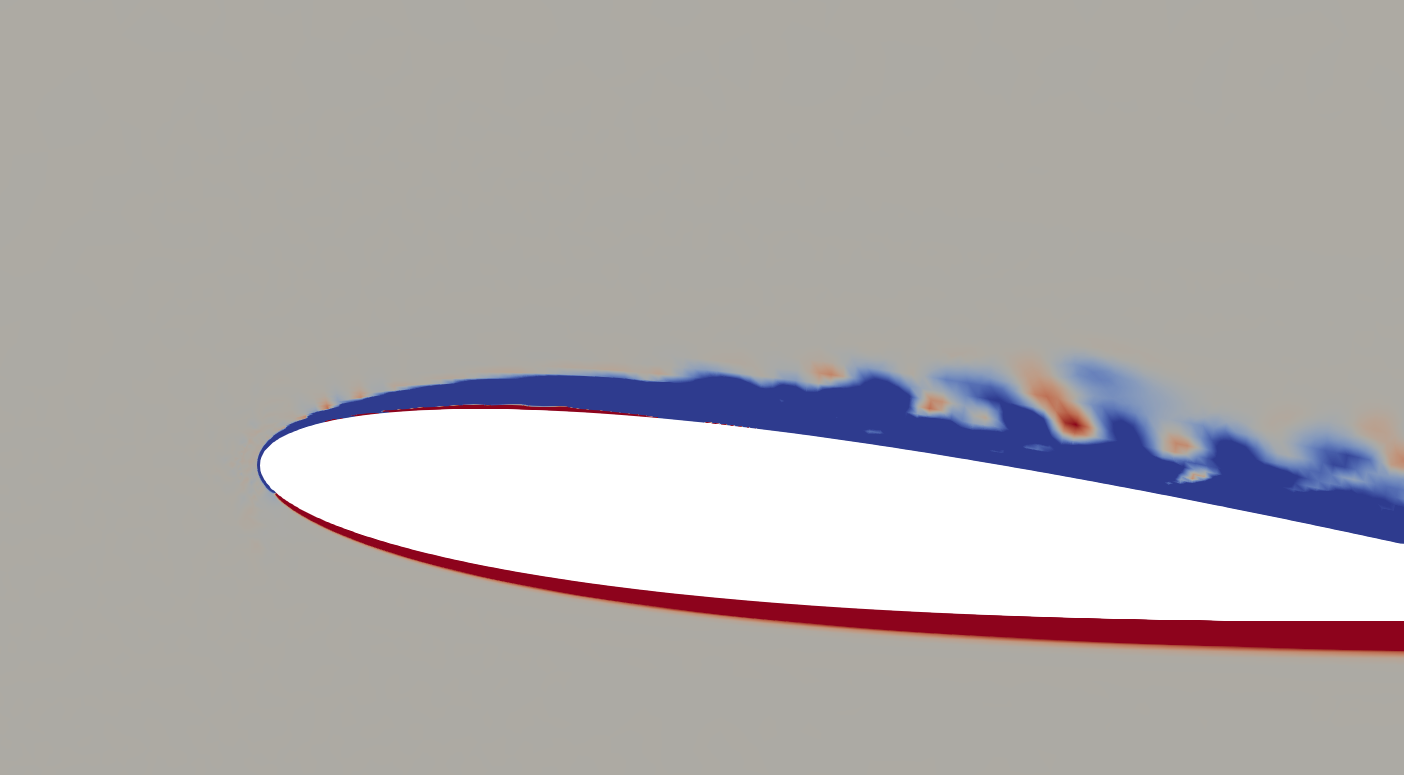
\includegraphics[width=1\textwidth]{figures/zonal_adapt_results/vorticity_plots/v2/Mza1_25/spavg/phase_180.png}
	\caption{Mza1\_nz25 mesh, $\psi$ = $180^\circ$}
	\label{fig:Mza1_25_sp_psi180}
\end{subfigure}
	\begin{subfigure}[b]{0.475\textwidth}
		\centering
		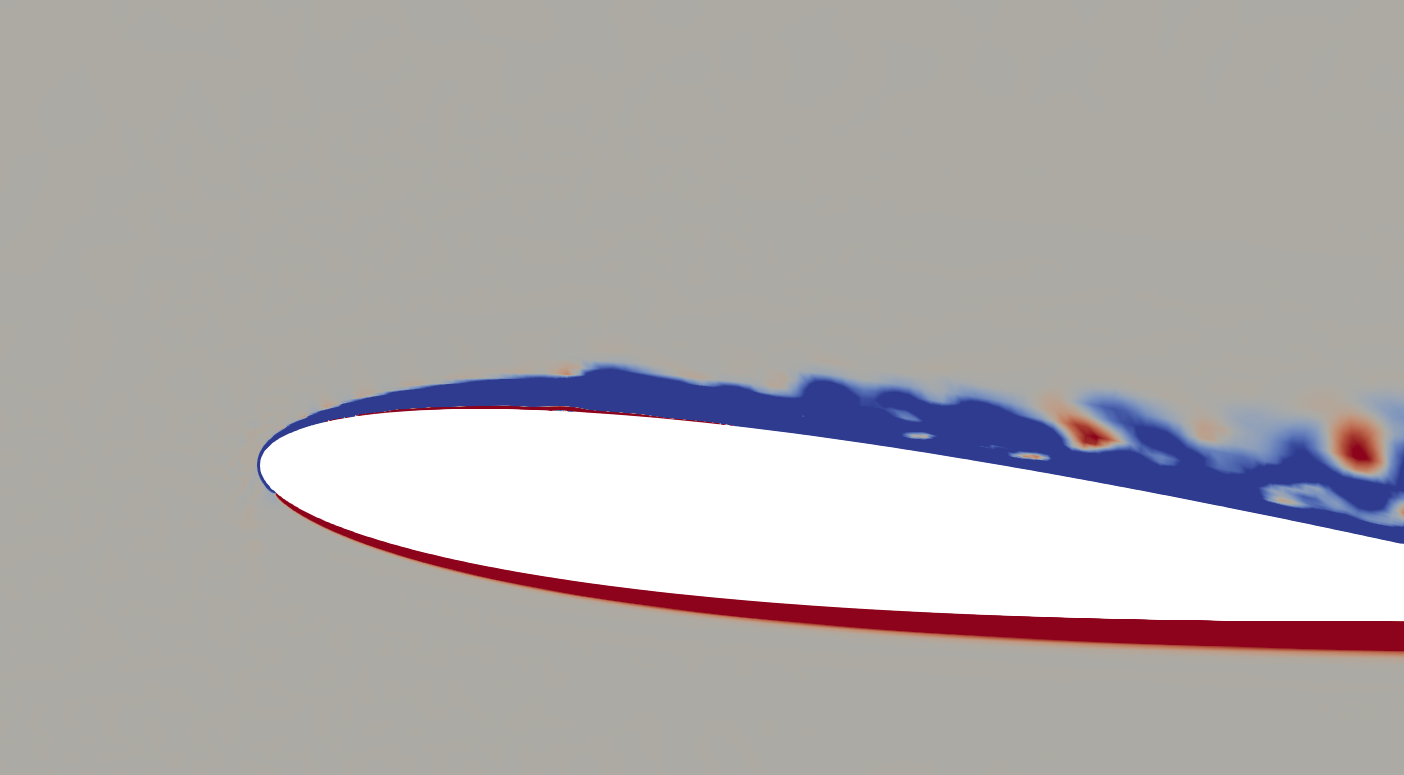
\includegraphics[width=1\textwidth]{figures/zonal_adapt_results/vorticity_plots/v2/Mza1_50/spavg/phase_180.png}
		\caption{Mza1\_nz50 mesh, $\psi$ = $180^\circ$}
		\label{fig:Mza1_50_sp_psi180}
	\end{subfigure}
%	\begin{subfigure}[b]{0.475\textwidth}
%		\centering
%		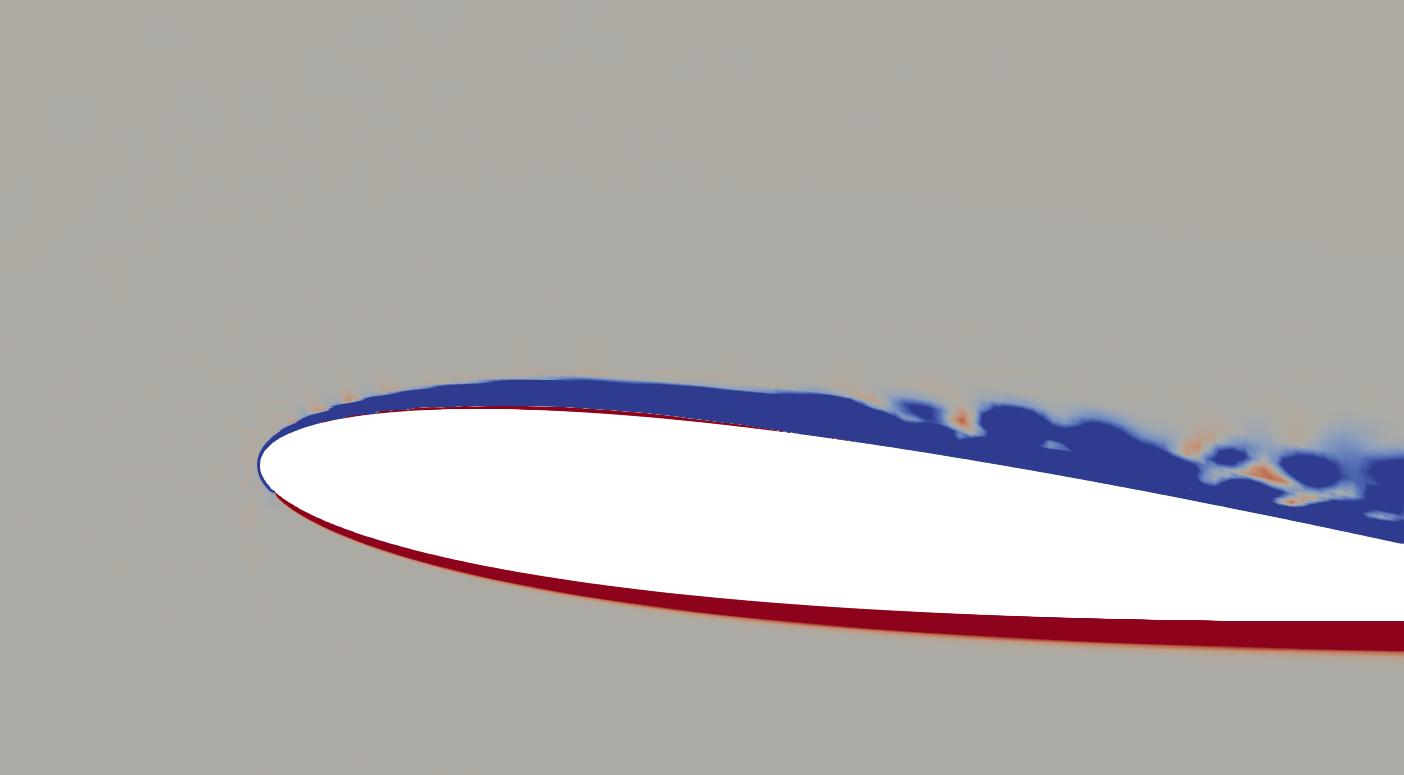
\includegraphics[width=1\textwidth]{figures/zonal_adapt_results/vorticity_plots/v2/Mza1_100/spavg/phase_180.png}
%		\caption{Mza1\_100 mesh, $\psi$ = $180^\circ$}
%		\label{fig:Mza1_100_sp_psi180}
%	\end{subfigure}
%	\begin{subfigure}[b]{0.475\textwidth}
%	\centering
%	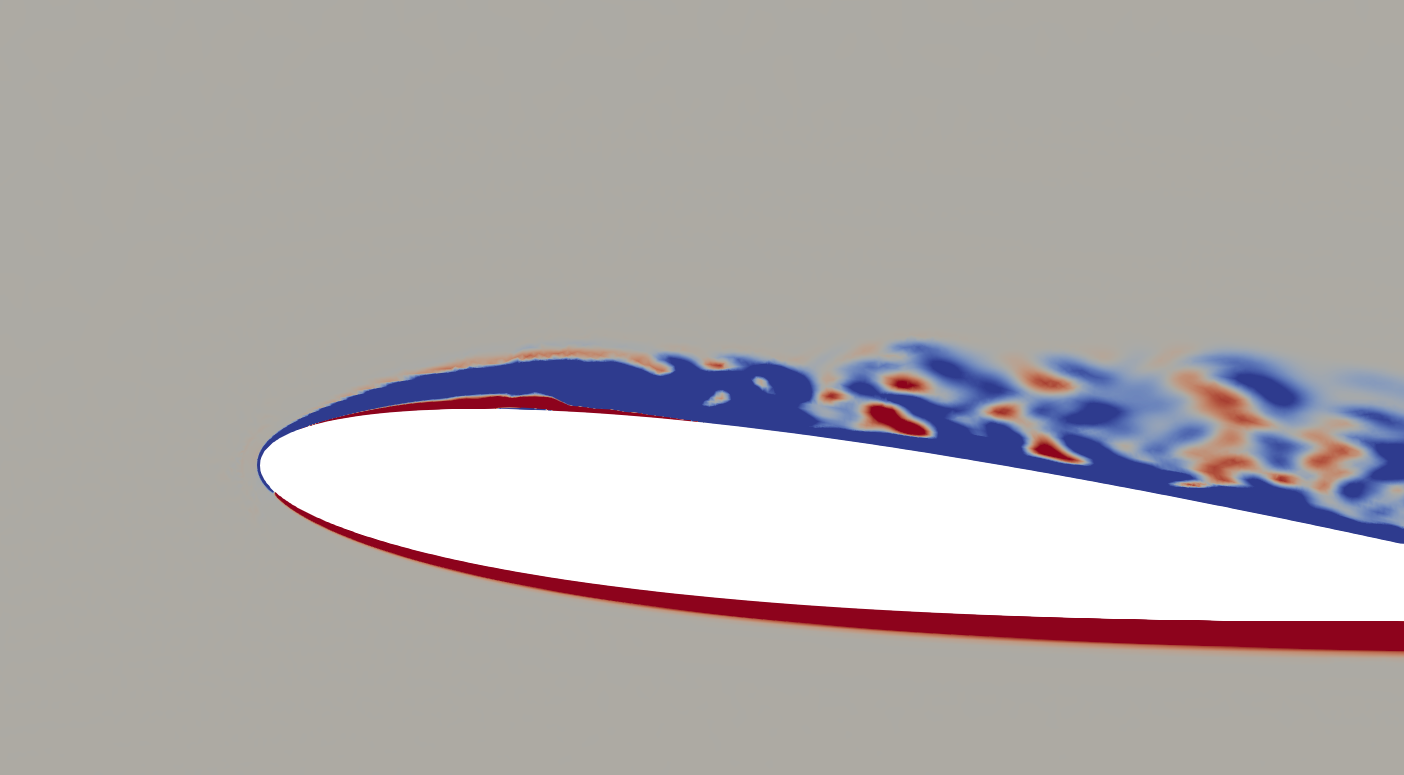
\includegraphics[width=1\textwidth]{figures/zonal_adapt_results/vorticity_plots/v2/Mza2_25/spavg/phase_180.png}
%	\caption{Mza2\_25 mesh, $\psi$ = $180^\circ$}
%	\label{fig:Mza2_25_sp_psi180}
%	\end{subfigure}
	\begin{subfigure}[b]{0.475\textwidth}
		\centering
		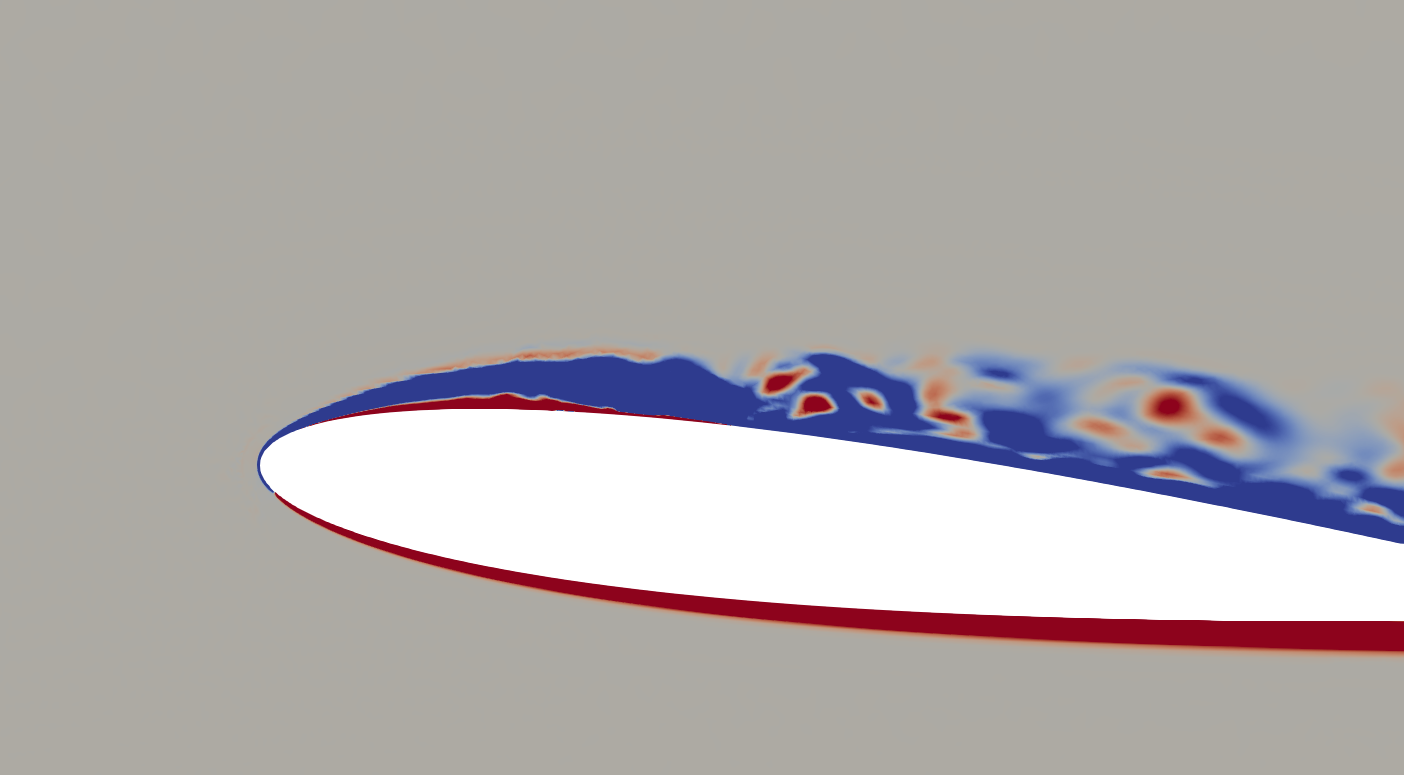
\includegraphics[width=1\textwidth]{figures/zonal_adapt_results/vorticity_plots/v2/Mza2_50/spavg/phase_180.png}
		\caption{Mza2\_nz50 mesh, $\psi$ = $180^\circ$}
		\label{fig:Mza2_50_sp_psi180}
	\end{subfigure}	
	\begin{subfigure}[b]{0.475\textwidth}
		\centering
		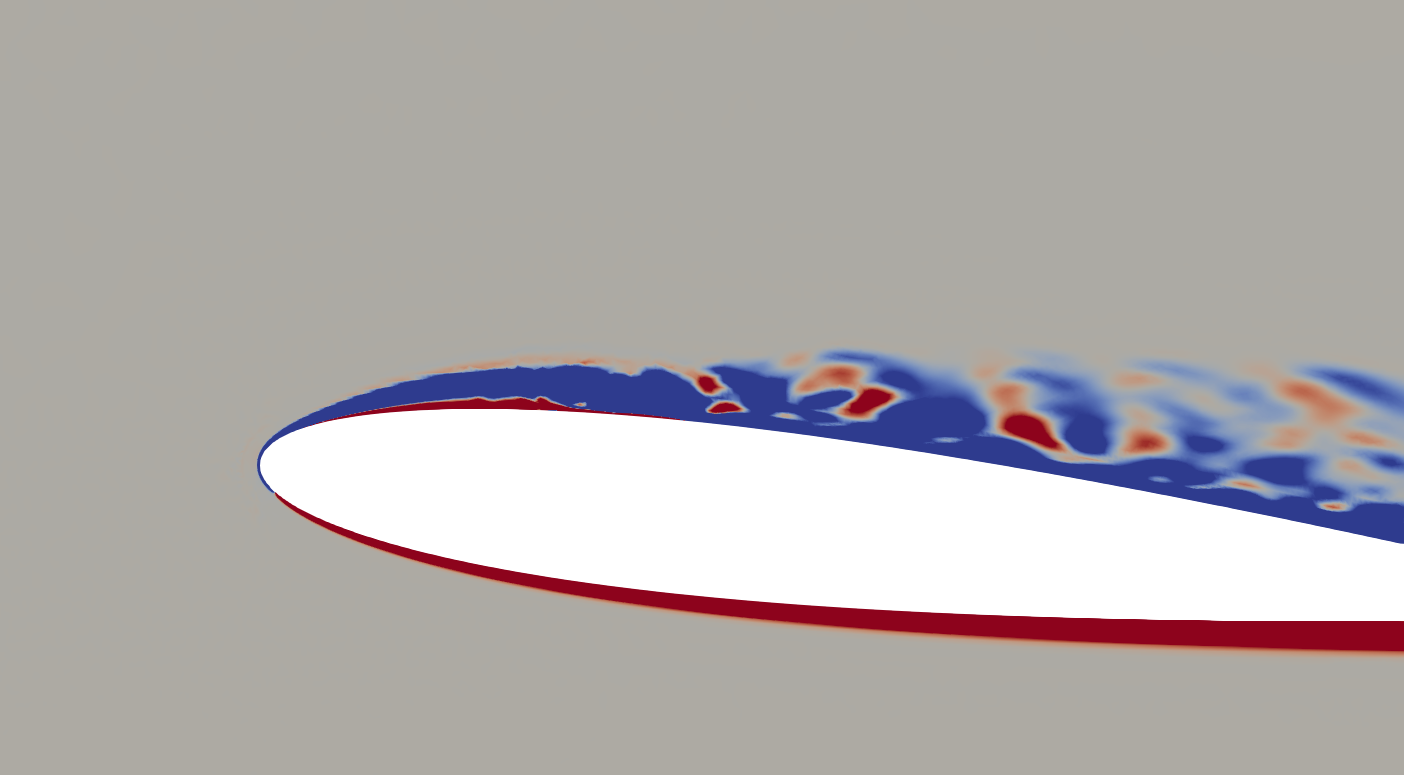
\includegraphics[width=1\textwidth]{figures/zonal_adapt_results/vorticity_plots/v2/Mza2_100/spavg/phase_180.png}
		\caption{Mza2\_nz100 mesh, $\psi$ = $180^\circ$}
		\label{fig:Mza2_100_sp_psi180}
	\end{subfigure}
	\begin{subfigure}[b]{0.475\textwidth}
	\centering
	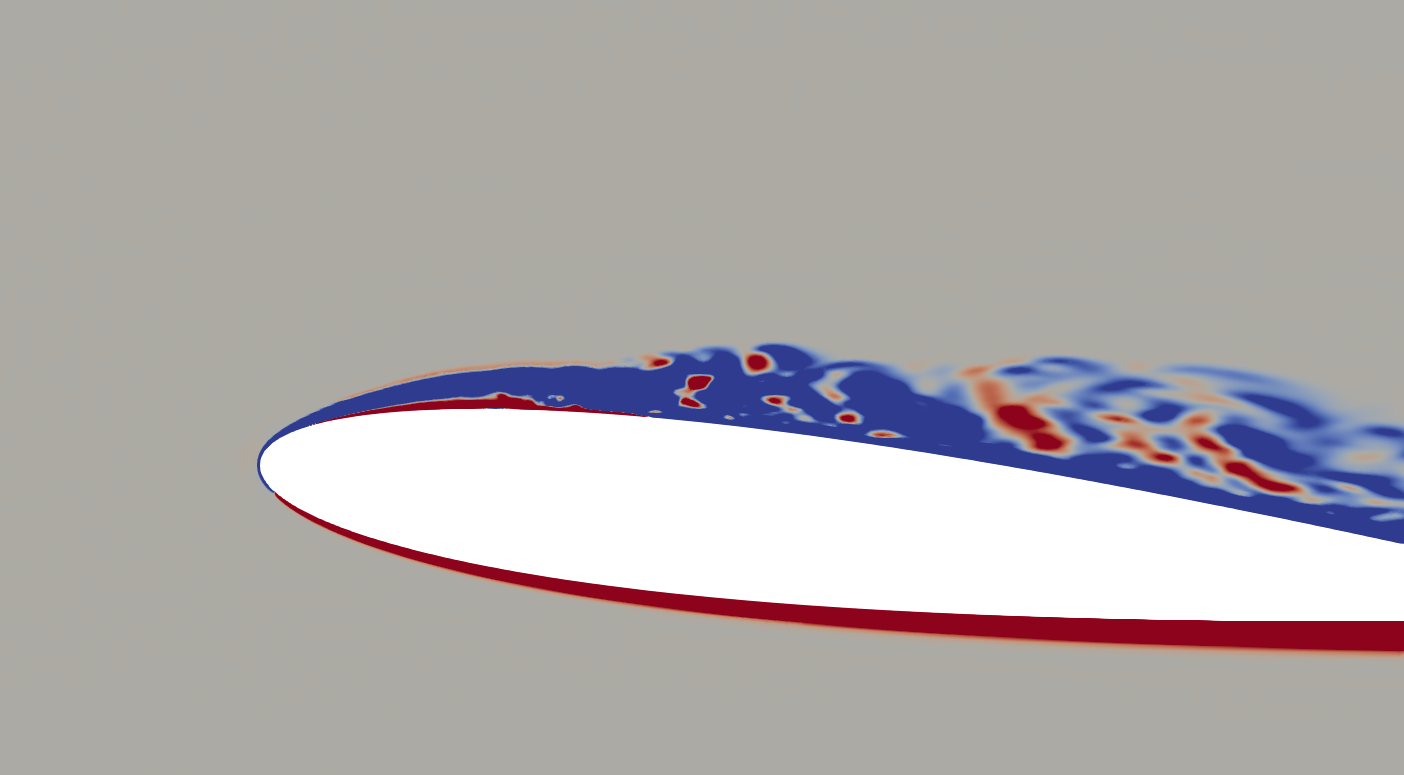
\includegraphics[width=1\textwidth]{figures/zonal_adapt_results/vorticity_plots/v2/Mza3_50/spavg/phase_180.png}
	\caption{Mza3\_nz50 mesh, $\psi$ = $180^\circ$}
	\label{fig:Mza3_50_sp_psi180}
	\end{subfigure}
	\begin{subfigure}[b]{0.475\textwidth}
		\centering
		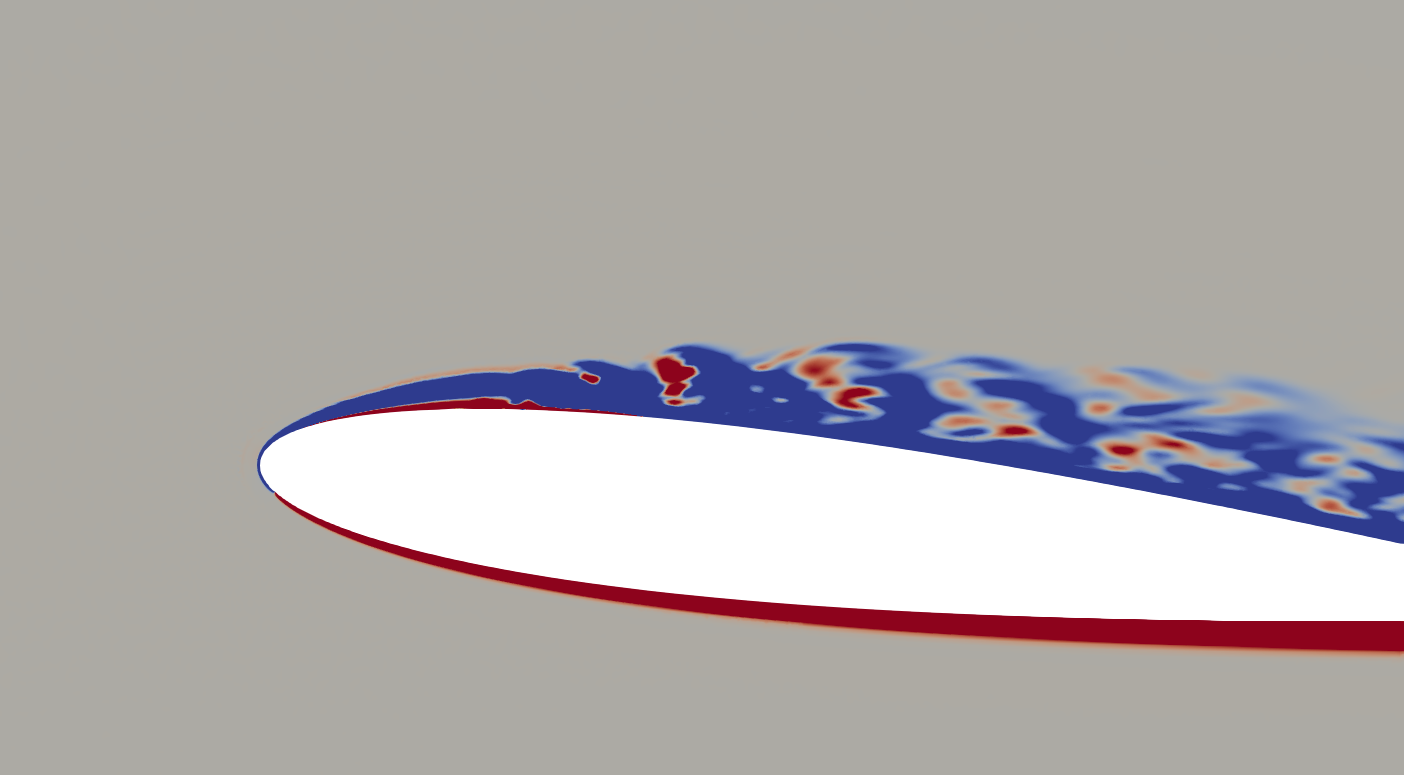
\includegraphics[width=1\textwidth]{figures/zonal_adapt_results/vorticity_plots/v2/Mza3_100/spavg/phase_180.png}
		\caption{Mza3\_nz100 mesh, $\psi$ = $180^\circ$}
		\label{fig:Mza3_100_sp_psi180}
	\end{subfigure}
	\caption{Spanwise vorticity comparison at $\psi$ = $180^\circ$ for different meshes}
	\label{fig:vorticity_zonal_180}
\end{figure}

%%=====================================
%% Phase = 210
%%=====================================


\begin{figure}[H]
	\centering
	\begin{center}
		\begin{subfigure}[b]{0.475\textwidth}
		\centering
		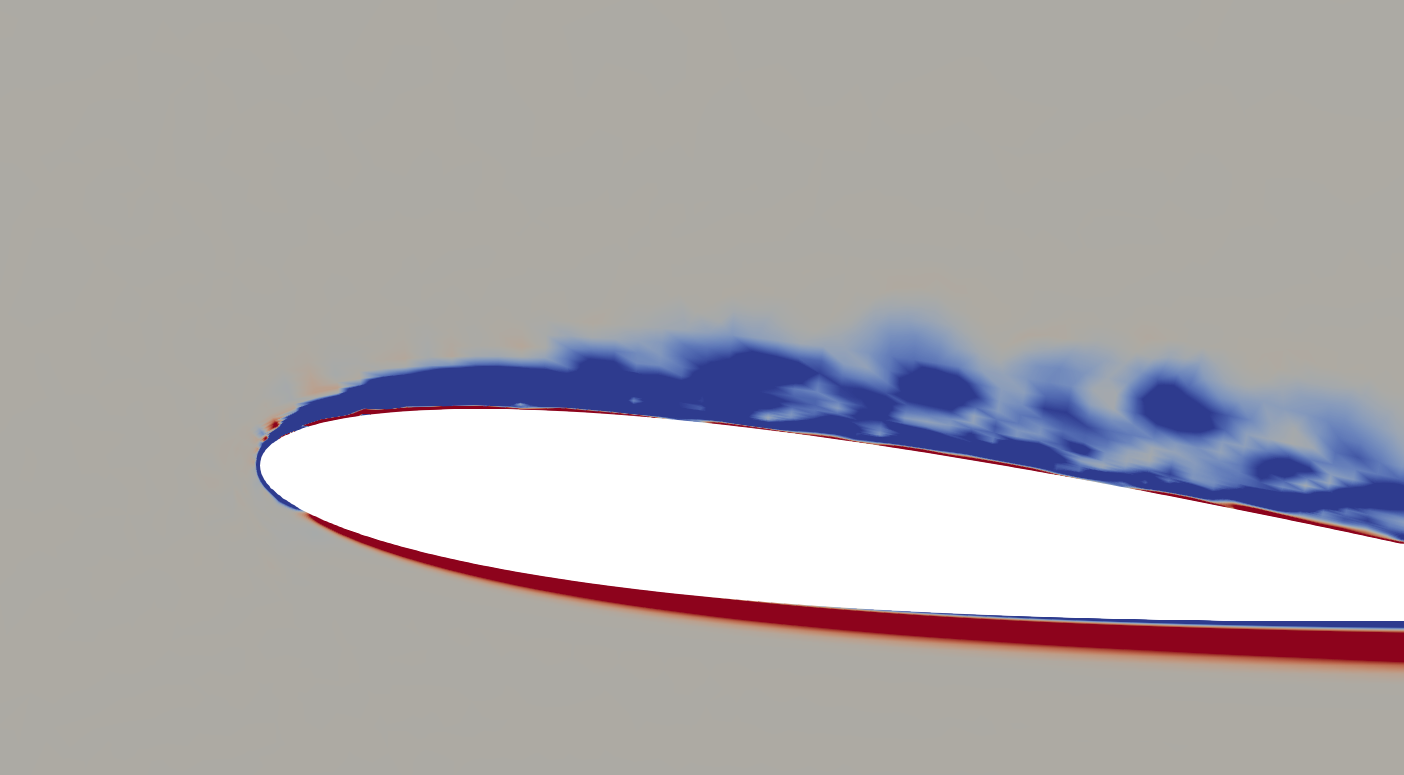
\includegraphics[width=1\textwidth]{figures/zonal_adapt_results/vorticity_plots/v2/M0/spavg/phase_210.png}
		\caption{M0\_nz25 mesh, $\psi$ = $210^\circ$}
		\label{fig:M0_sp_psi210}
		\end{subfigure}
	\end{center}
	\begin{subfigure}[b]{0.475\textwidth}
	\centering
	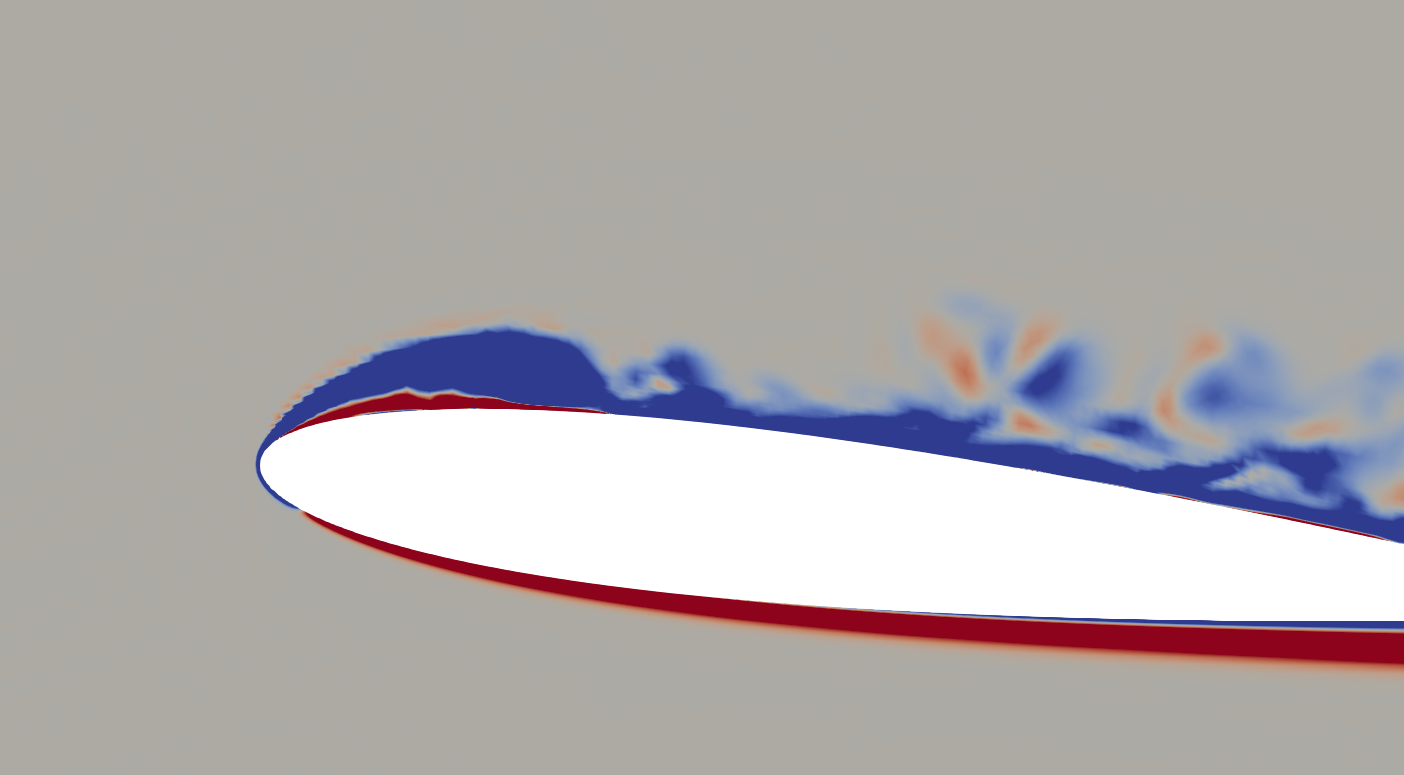
\includegraphics[width=1\textwidth]{figures/zonal_adapt_results/vorticity_plots/v2/Mza1_25/spavg/phase_210.png}
	\caption{Mza1\_nz25 mesh, $\psi$ = $210^\circ$}
	\label{fig:Mza1_25_sp_psi210}
	\end{subfigure}
	\begin{subfigure}[b]{0.475\textwidth}
		\centering
		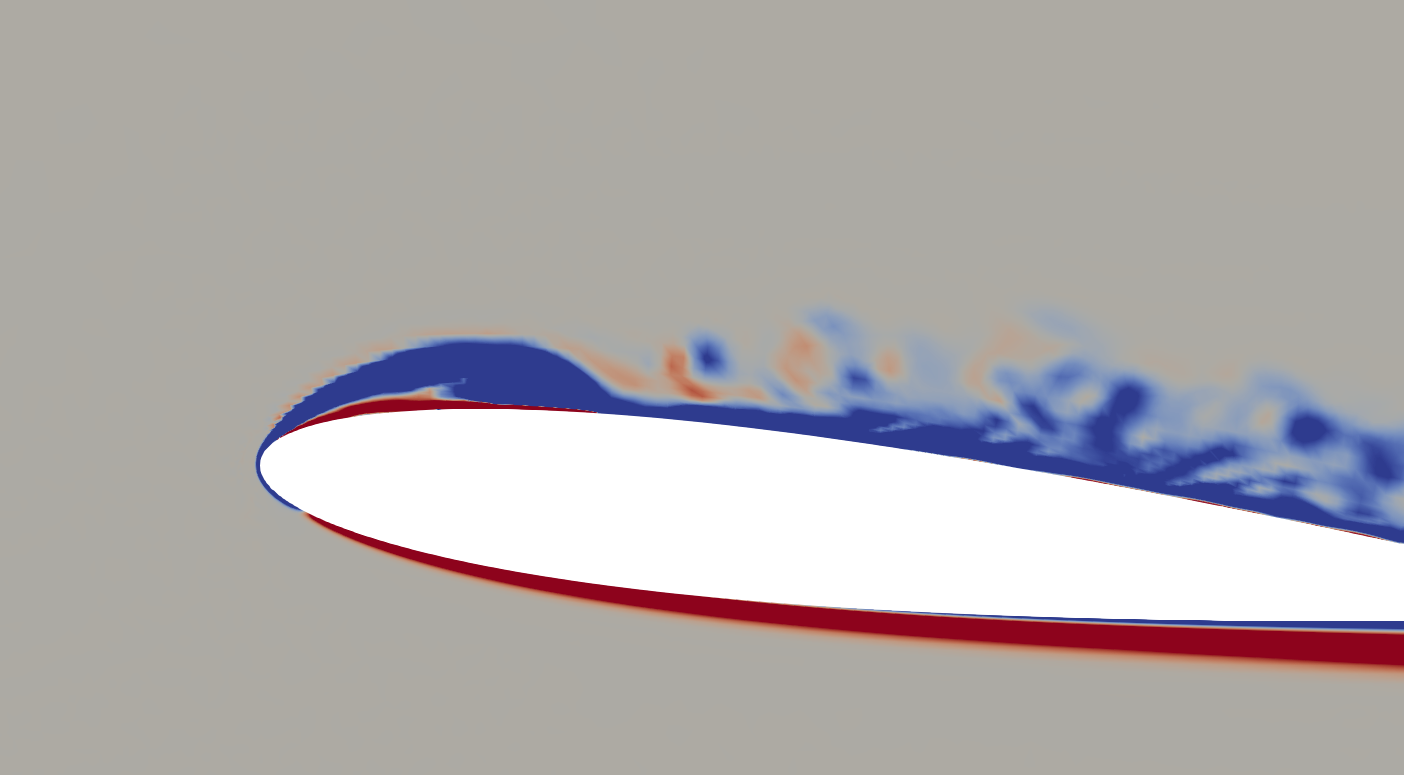
\includegraphics[width=1\textwidth]{figures/zonal_adapt_results/vorticity_plots/v2/Mza1_50/spavg/phase_210.png}
		\caption{Mza1\_nz50 mesh, $\psi$ = $210^\circ$}
		\label{fig:Mza1_50_sp_psi210}
	\end{subfigure}
%	\begin{subfigure}[b]{0.475\textwidth}
%		\centering
%		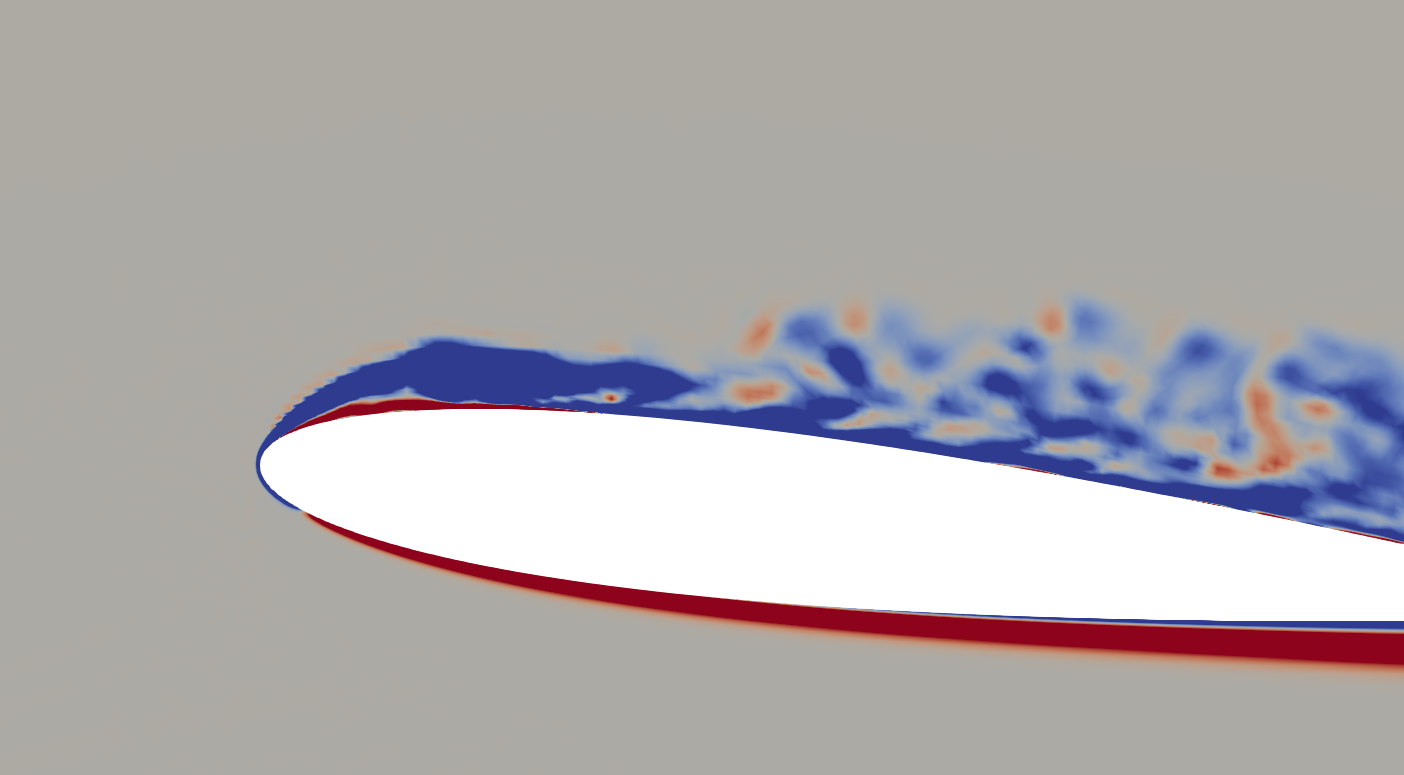
\includegraphics[width=1\textwidth]{figures/zonal_adapt_results/vorticity_plots/v2/Mza1_100/spavg/phase_210.png}
%		\caption{Mza1\_100 mesh, $\psi$ = $210^\circ$}
%		\label{fig:Mza1_100_sp_psi210}
%	\end{subfigure}
%	\begin{subfigure}[b]{0.475\textwidth}
%	\centering
%	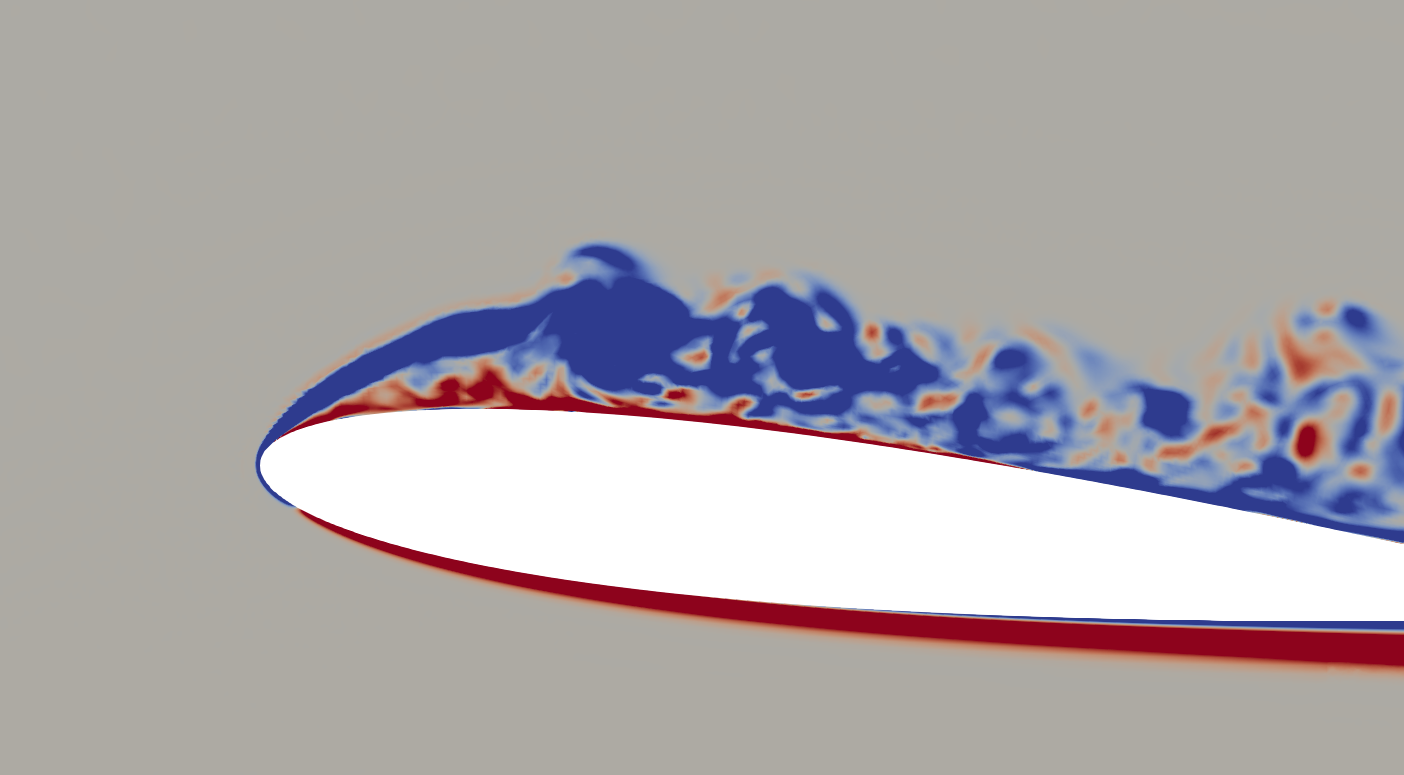
\includegraphics[width=1\textwidth]{figures/zonal_adapt_results/vorticity_plots/v2/Mza2_25/spavg/phase_210.png}
%	\caption{Mza2\_25 mesh, $\psi$ = $210^\circ$}
%	\label{fig:Mza2_25_sp_psi210}
%	\end{subfigure}	
	\begin{subfigure}[b]{0.475\textwidth}
		\centering
		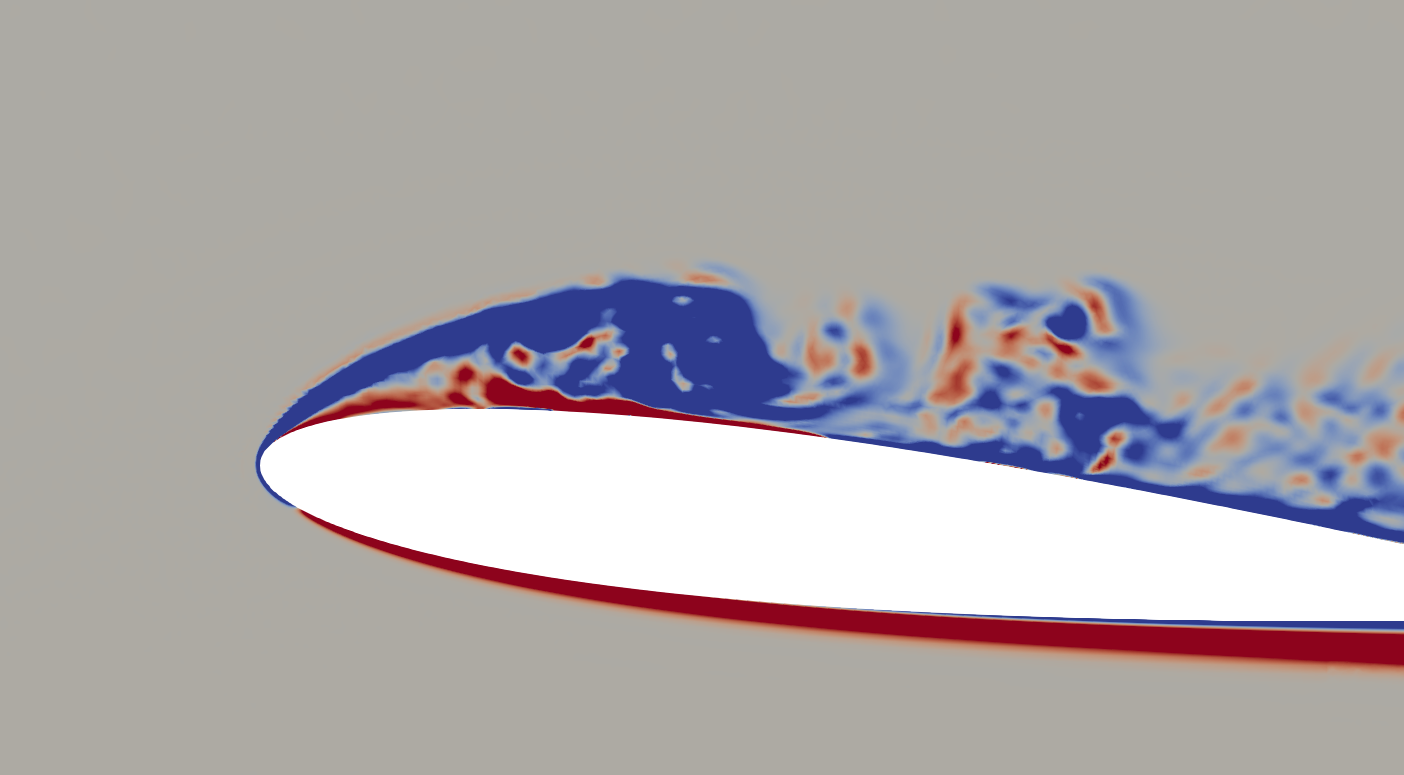
\includegraphics[width=1\textwidth]{figures/zonal_adapt_results/vorticity_plots/v2/Mza2_50/spavg/phase_210.png}
		\caption{Mza2\_nz50 mesh, $\psi$ = $210^\circ$}
		\label{fig:Mza2_50_sp_psi210}
	\end{subfigure}	
	\begin{subfigure}[b]{0.475\textwidth}
		\centering
		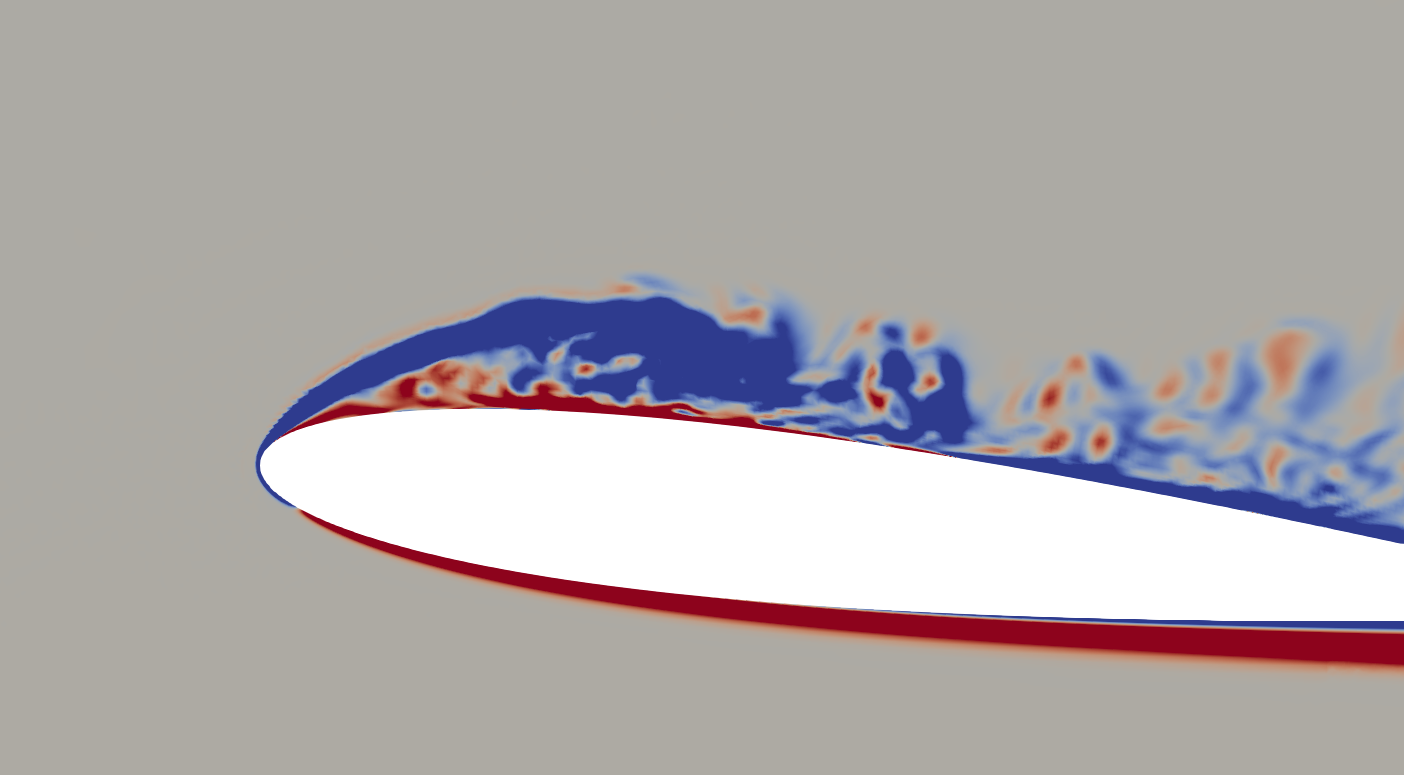
\includegraphics[width=1\textwidth]{figures/zonal_adapt_results/vorticity_plots/v2/Mza2_100/spavg/phase_210.png}
		\caption{Mza2\_nz100 mesh, $\psi$ = $210^\circ$}
		\label{fig:Mza2_100_sp_psi210}
	\end{subfigure}
	\begin{subfigure}[b]{0.475\textwidth}
	\centering
	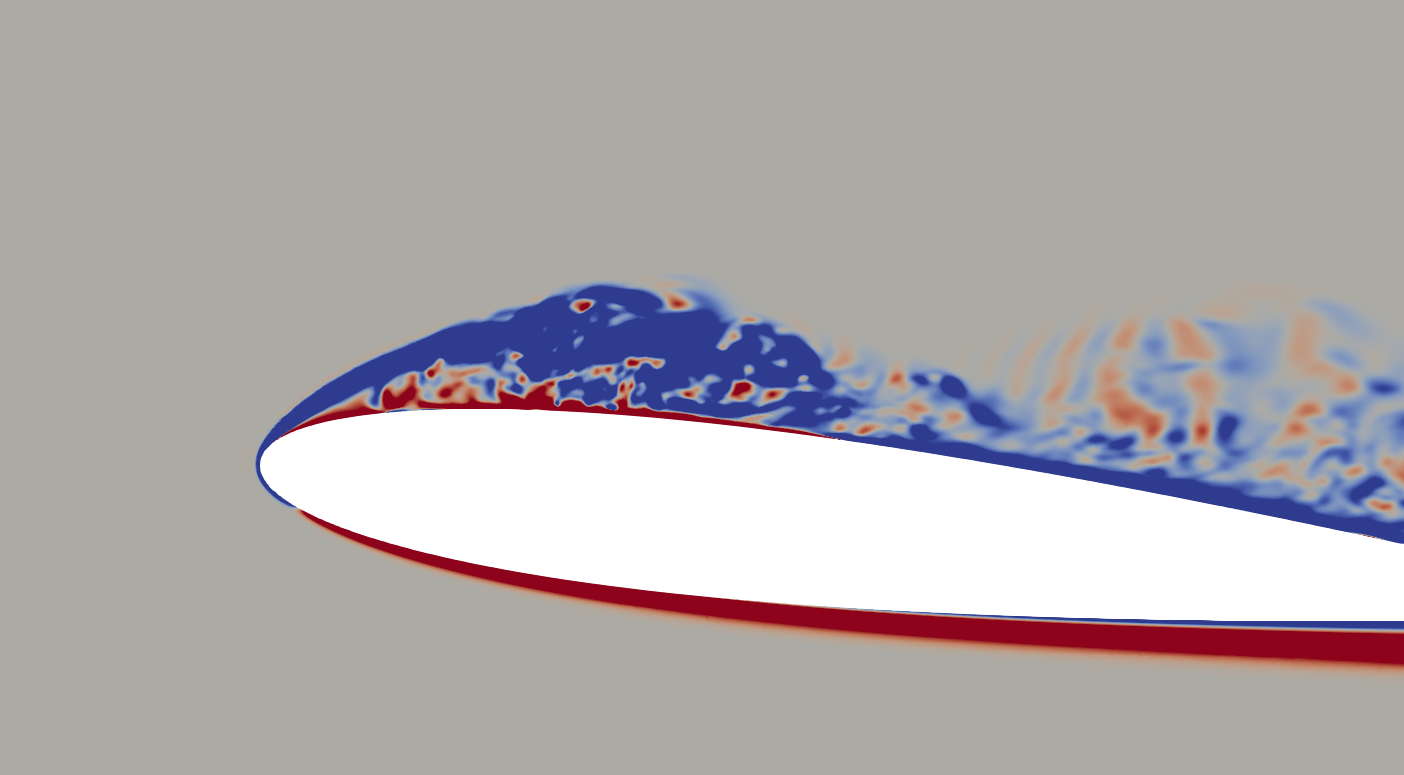
\includegraphics[width=1\textwidth]{figures/zonal_adapt_results/vorticity_plots/v2/Mza3_50/spavg/phase_210.png}
	\caption{Mza3\_nz50 mesh, $\psi$ = $210^\circ$}
	\label{fig:Mza3_50_sp_psi210}
\end{subfigure}
	\begin{subfigure}[b]{0.475\textwidth}
		\centering
		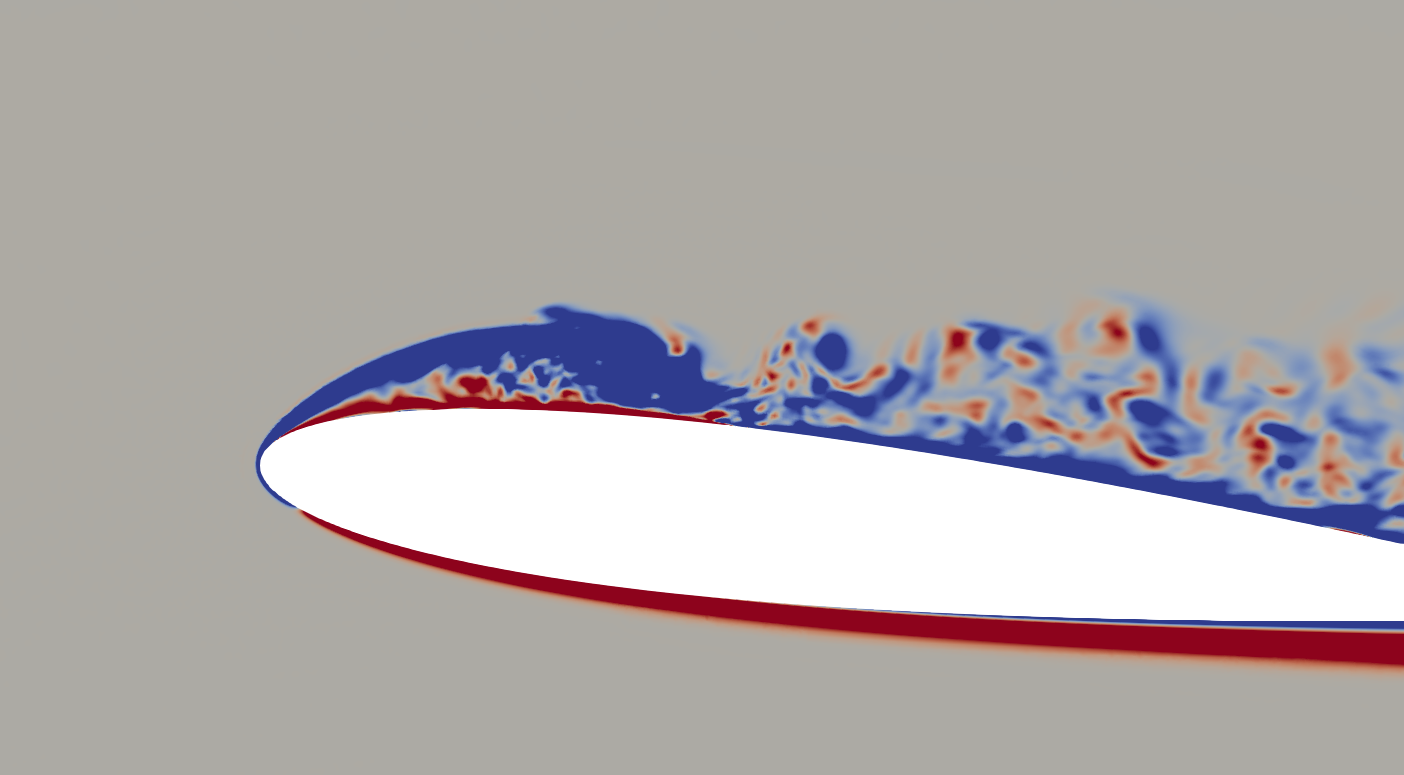
\includegraphics[width=1\textwidth]{figures/zonal_adapt_results/vorticity_plots/v2/Mza3_100/spavg/phase_210.png}
		\caption{Mza3\_nz100 mesh, $\psi$ = $210^\circ$}
		\label{fig:Mza3_100_sp_psi210}
	\end{subfigure}
	\caption{Spanwise vorticity comparison at $\psi$ = $210^\circ$ for different meshes}
	\label{fig:vorticity_zonal_210}
\end{figure}

%%=====================================
%% Phase = 240
%%=====================================


\begin{figure}[H]
	\centering
	\begin{center}
		\begin{subfigure}[b]{0.475\textwidth}
		\centering
		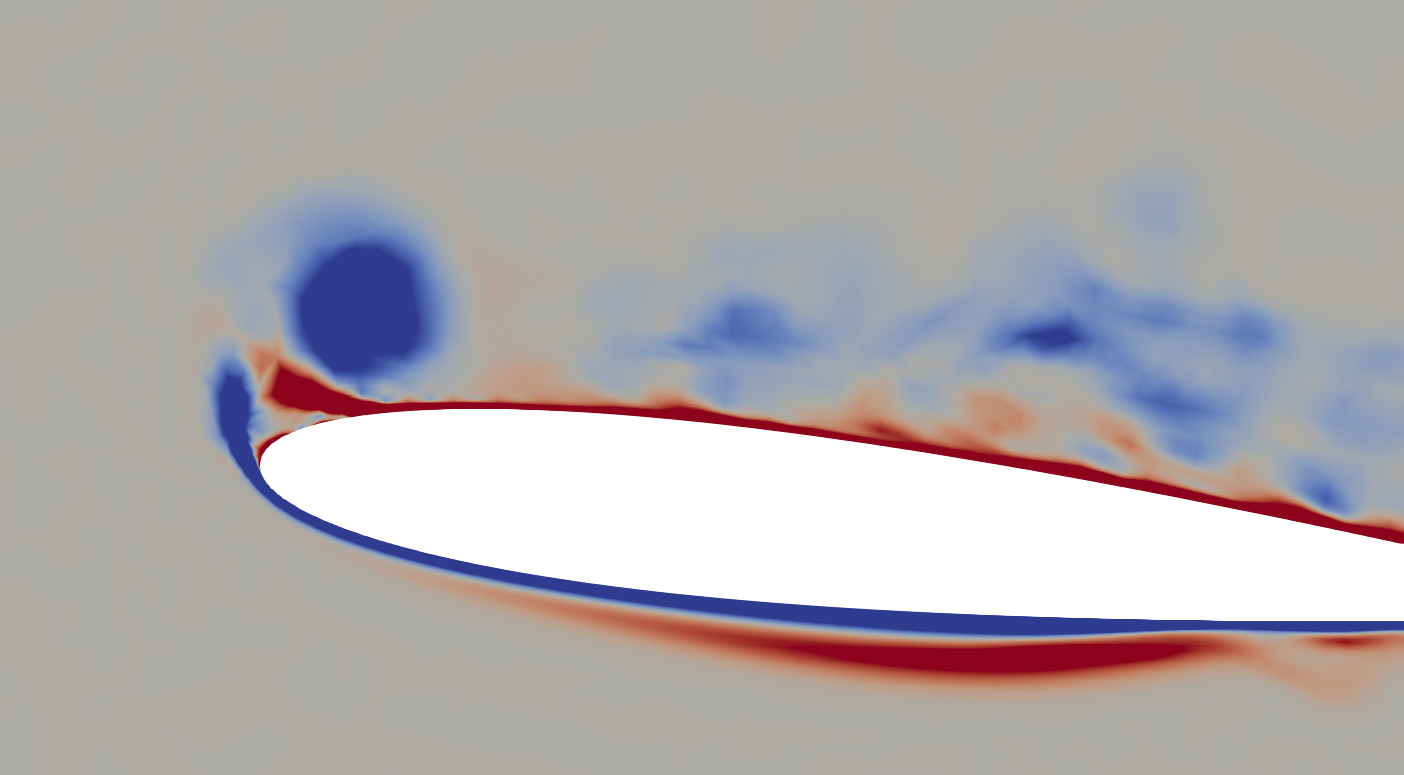
\includegraphics[width=1\textwidth]{figures/zonal_adapt_results/vorticity_plots/v2/M0/spavg/phase_240.png}
		\caption{M0\_nz25 mesh, $\psi$ = $240^\circ$}
		\label{fig:M0_sp_psi240}
		\end{subfigure}
	\end{center}
	\begin{subfigure}[b]{0.475\textwidth}
		\centering
		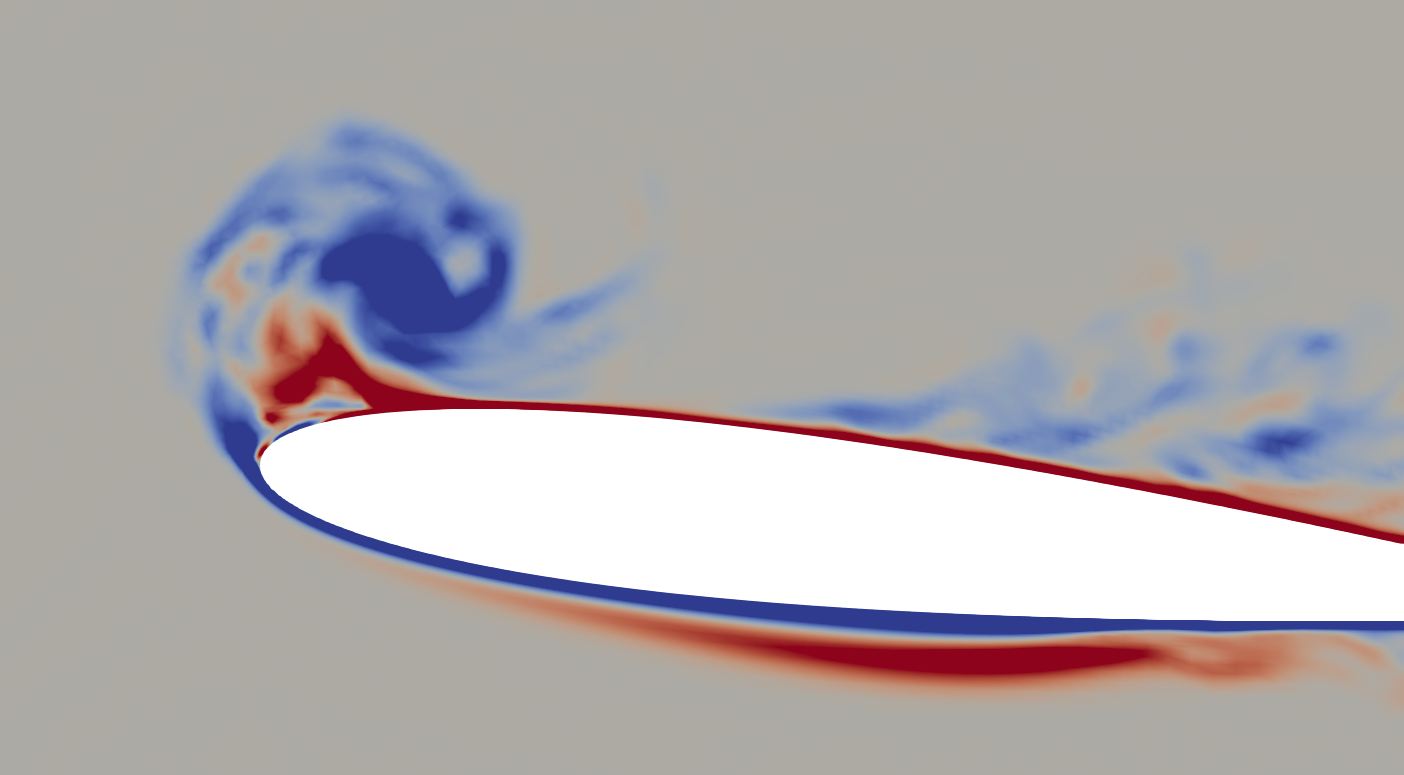
\includegraphics[width=1\textwidth]{figures/zonal_adapt_results/vorticity_plots/v2/Mza1_25/spavg/phase_240.png}
		\caption{Mza1\_nz25 mesh, $\psi$ = $240^\circ$}
		\label{fig:Mza1_25_sp_psi240}
	\end{subfigure}
	\begin{subfigure}[b]{0.475\textwidth}
	\centering
	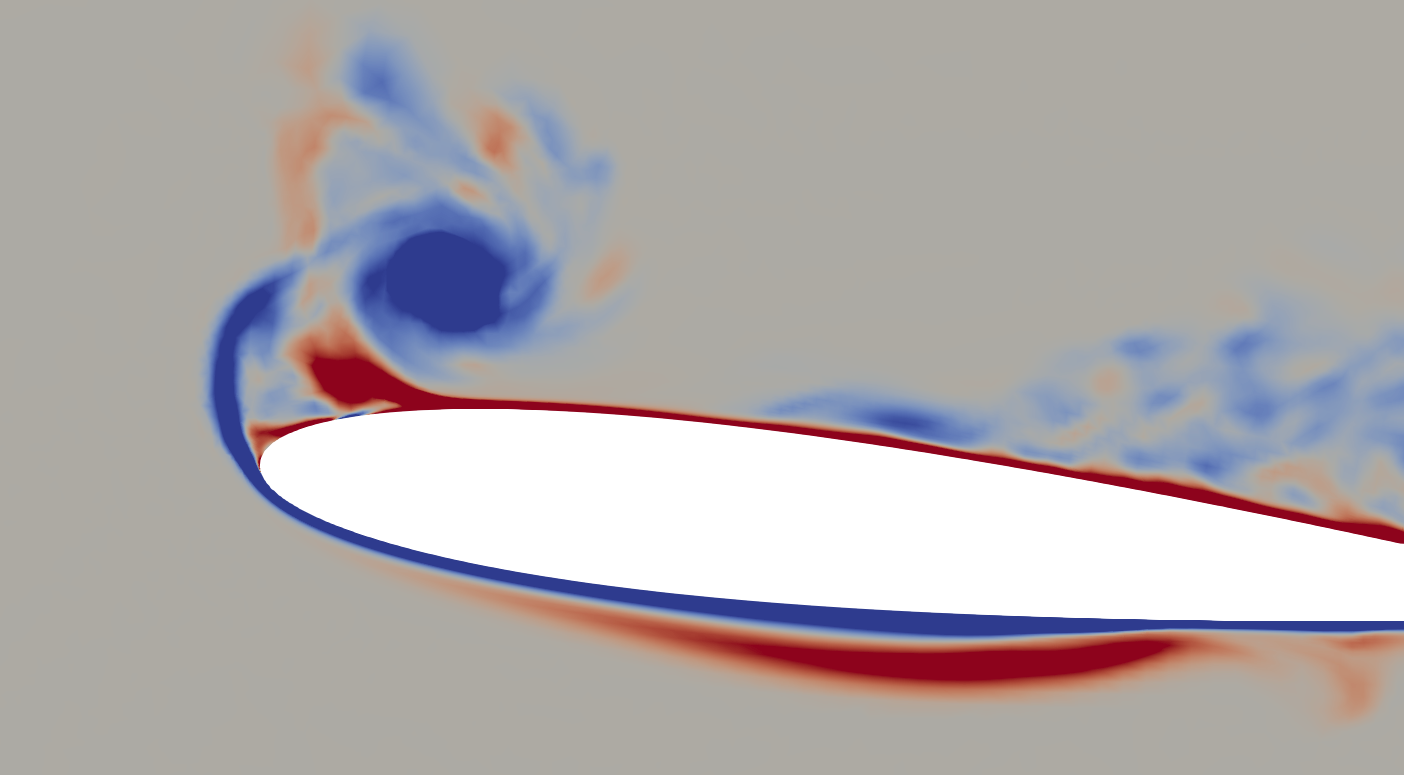
\includegraphics[width=1\textwidth]{figures/zonal_adapt_results/vorticity_plots/v2/Mza1_50/spavg/phase_240.png}
	\caption{Mza1\_nz50 mesh, $\psi$ = $240^\circ$}
	\label{fig:Mza1_50_sp_psi240}
	\end{subfigure}
	\begin{subfigure}[b]{0.475\textwidth}
		\centering
		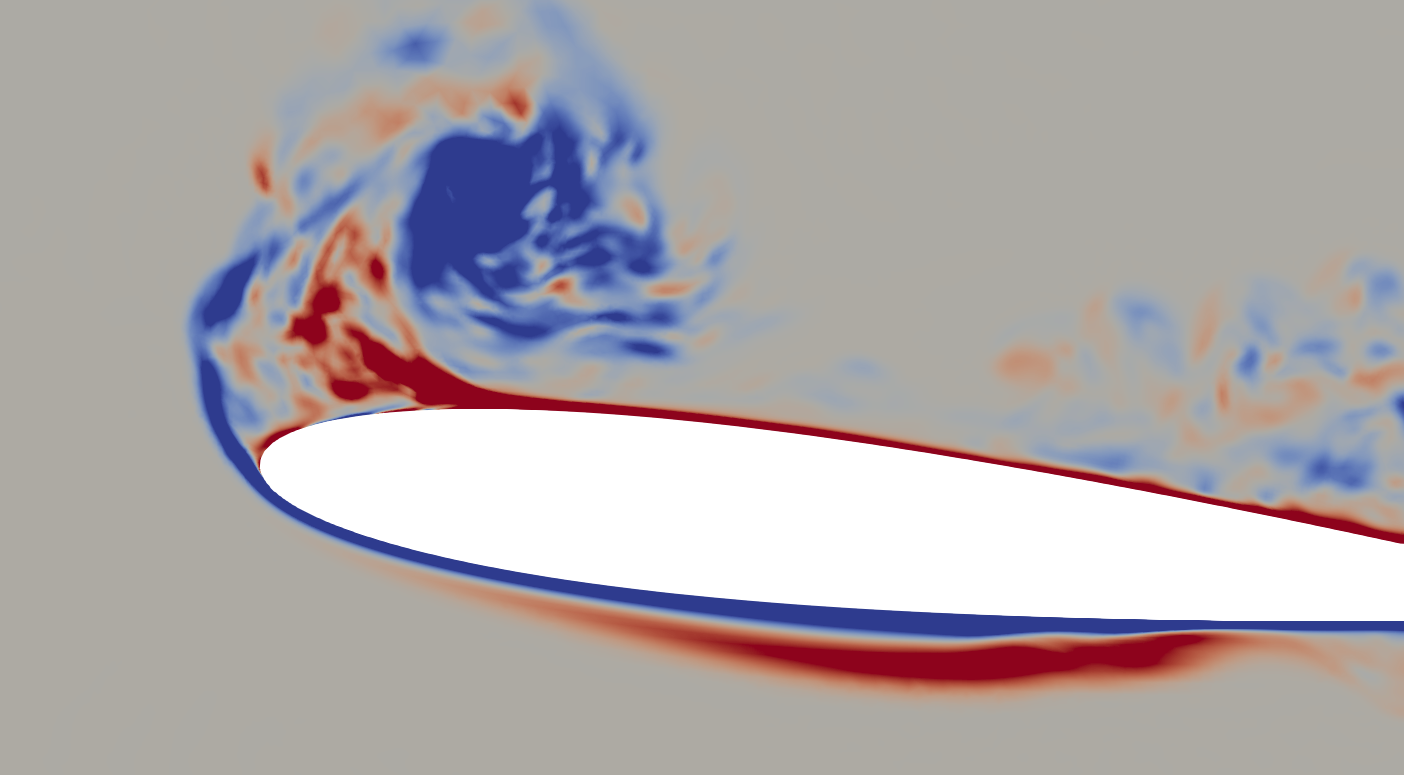
\includegraphics[width=1\textwidth]{figures/zonal_adapt_results/vorticity_plots/v2/Mza2_50/spavg/phase_240.png}
		\caption{Mza2\_nz50 mesh, $\psi$ = $240^\circ$}
		\label{fig:Mza2_50_sp_psi240}
	\end{subfigure}
%	\begin{subfigure}[b]{0.475\textwidth}
%		\centering
%		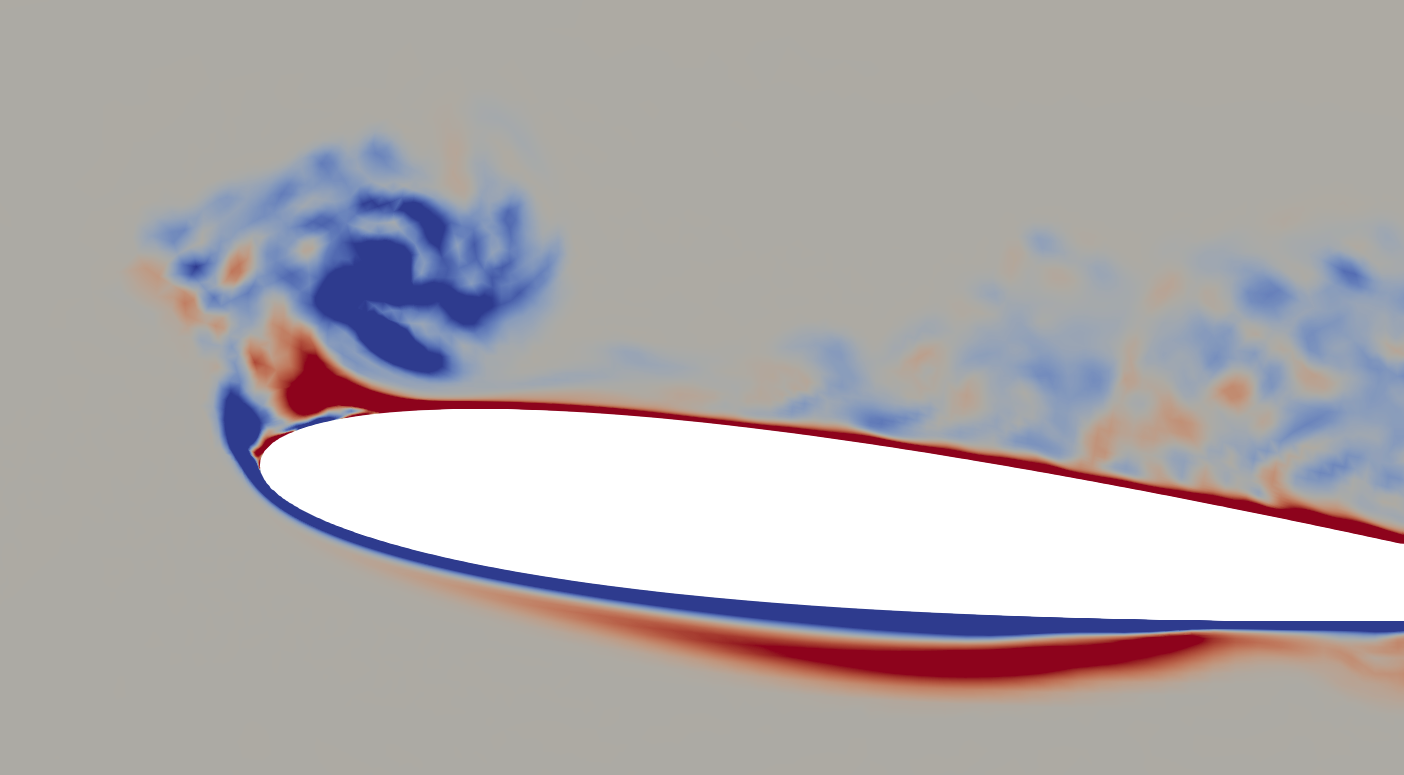
\includegraphics[width=1\textwidth]{figures/zonal_adapt_results/vorticity_plots/v2/Mza1_100/spavg/phase_240.png}
%		\caption{Mza1\_100 mesh, $\psi$ = $240^\circ$}
%		\label{fig:Mza1_100_sp_psi240}
%	\end{subfigure}
%	\begin{subfigure}[b]{0.475\textwidth}
%	\centering
%	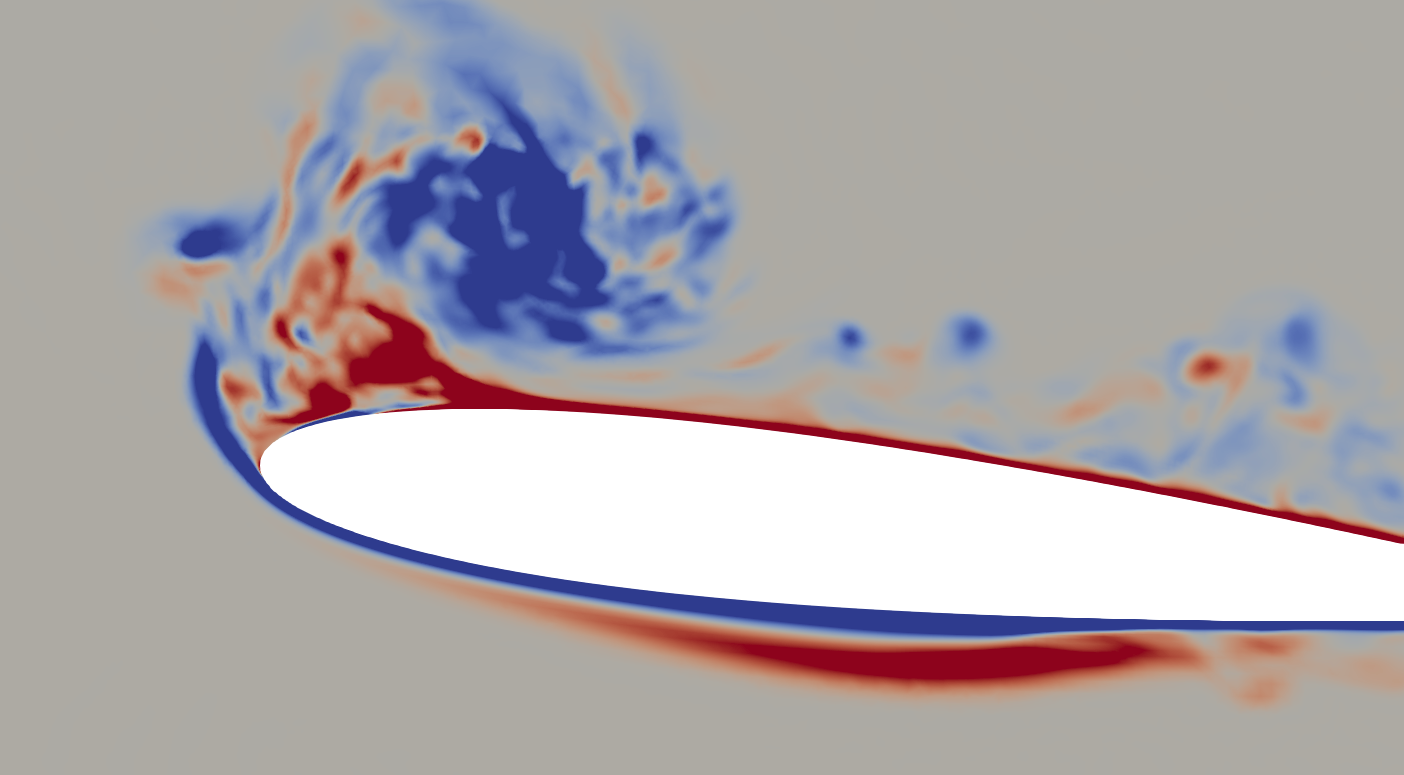
\includegraphics[width=1\textwidth]{figures/zonal_adapt_results/vorticity_plots/v2/Mza2_25/spavg/phase_240.png}
%	\caption{Mza2\_25 mesh, $\psi$ = $240^\circ$}
%	\label{fig:Mza2_25_sp_psi240}
%	\end{subfigure}	
%	\begin{subfigure}[b]{0.475\textwidth}
%		\centering
%		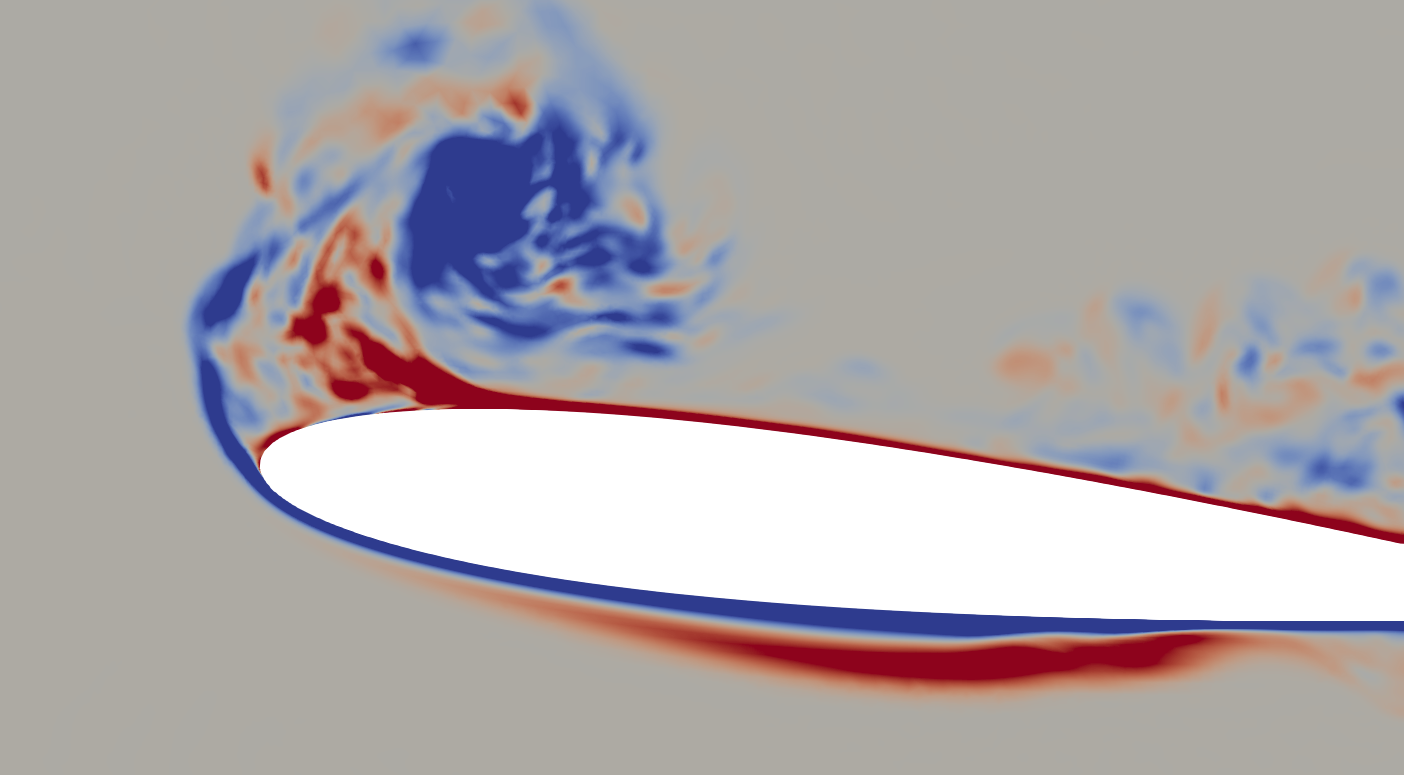
\includegraphics[width=1\textwidth]{figures/zonal_adapt_results/vorticity_plots/v2/Mza2_50/spavg/phase_240.png}
%		\caption{Mza2\_nz50 mesh, $\psi$ = $240^\circ$}
%		\label{fig:Mza2_50_sp_psi240}
%	\end{subfigure}	
	\begin{subfigure}[b]{0.475\textwidth}
		\centering
		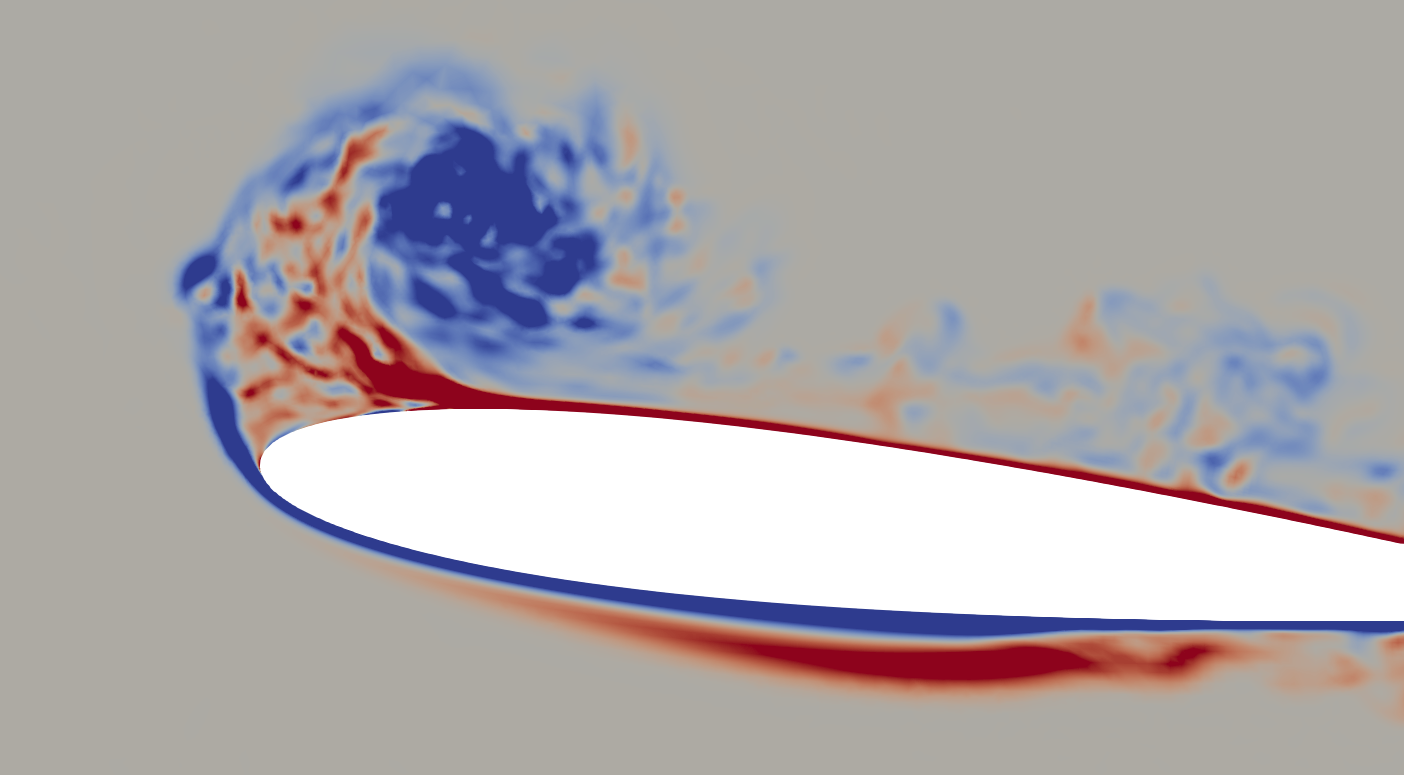
\includegraphics[width=1\textwidth]{figures/zonal_adapt_results/vorticity_plots/v2/Mza2_100/spavg/phase_240.png}
		\caption{Mza2\_nz100 mesh, $\psi$ = $240^\circ$}
		\label{fig:Mza2_100_sp_psi240}
	\end{subfigure}
	\begin{subfigure}[b]{0.475\textwidth}
	\centering
	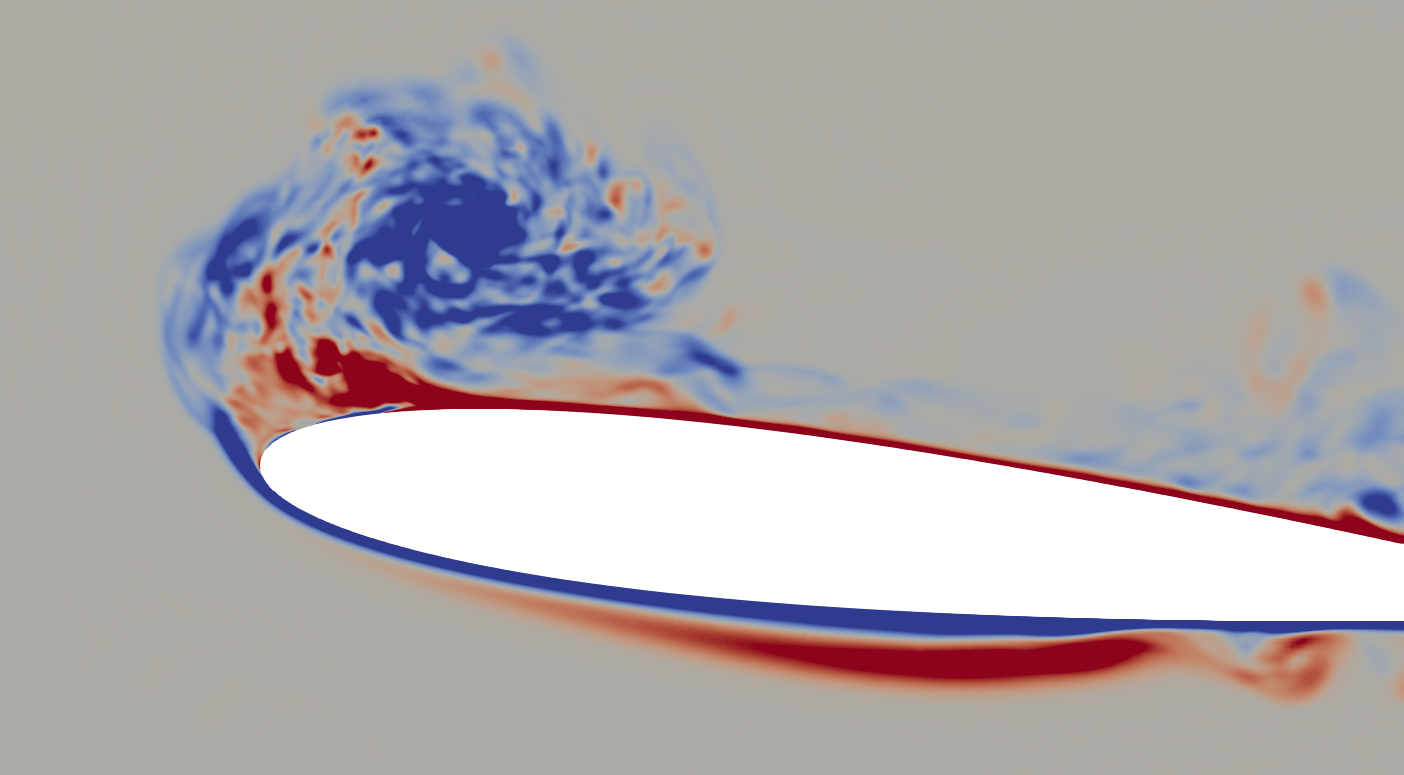
\includegraphics[width=1\textwidth]{figures/zonal_adapt_results/vorticity_plots/v2/Mza3_50/spavg/phase_240.png}
	\caption{Mza3\_nz50 mesh, $\psi$ = $240^\circ$}
	\label{fig:Mza3_50_sp_psi240}
\end{subfigure}
	\begin{subfigure}[b]{0.475\textwidth}
		\centering
		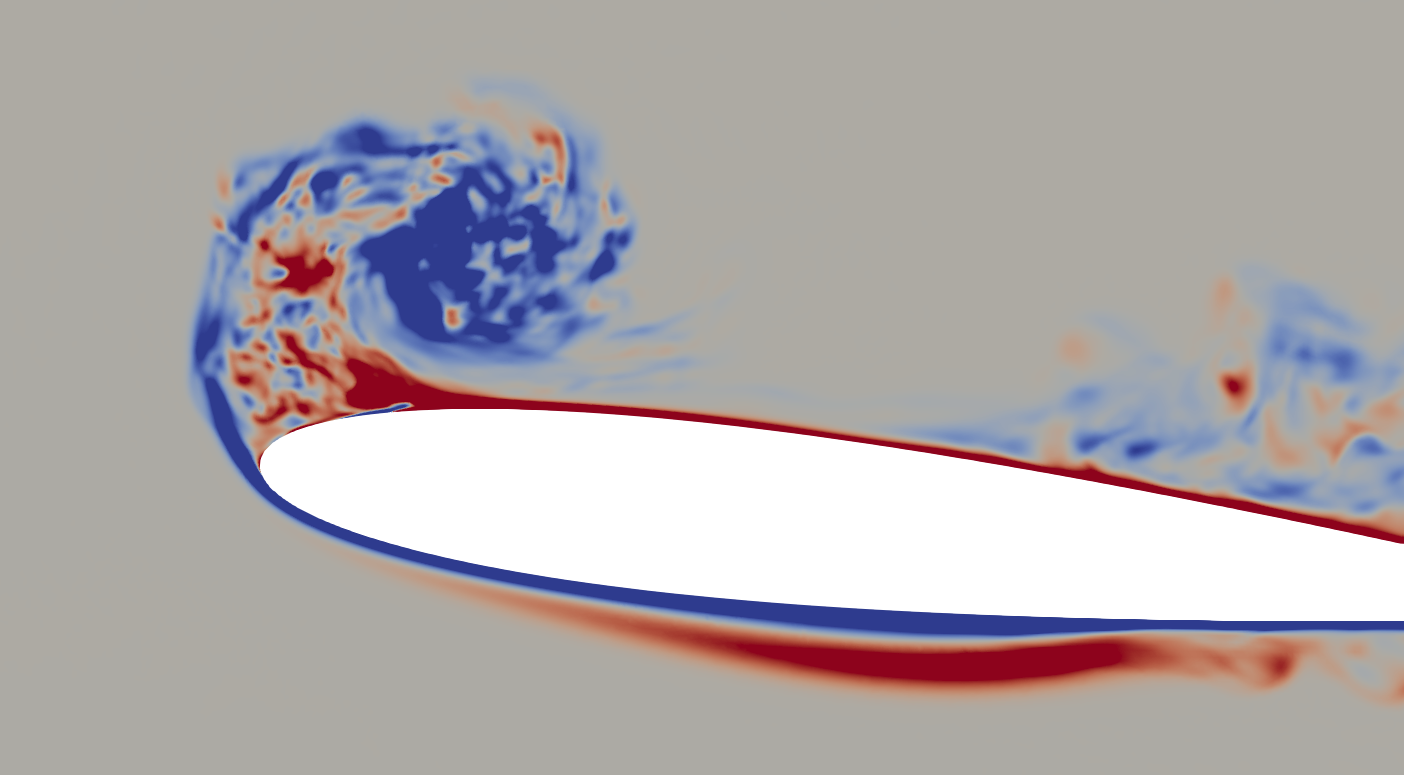
\includegraphics[width=1\textwidth]{figures/zonal_adapt_results/vorticity_plots/v2/Mza3_100/spavg/phase_240.png}
		\caption{Mza3\_nz100 mesh, $\psi$ = $240^\circ$}
		\label{fig:Mza3_100_sp_psi240}
	\end{subfigure}
	\caption{Spanwise vorticity comparison at $\psi$ = $240^\circ$ for different meshes}
	\label{fig:vorticity_zonal_240}
\end{figure}

%%=====================================
%% Phase = 270
%%=====================================


\begin{figure}[H]
	\centering
	\begin{center}
		\begin{subfigure}[b]{0.475\textwidth}
		\centering
		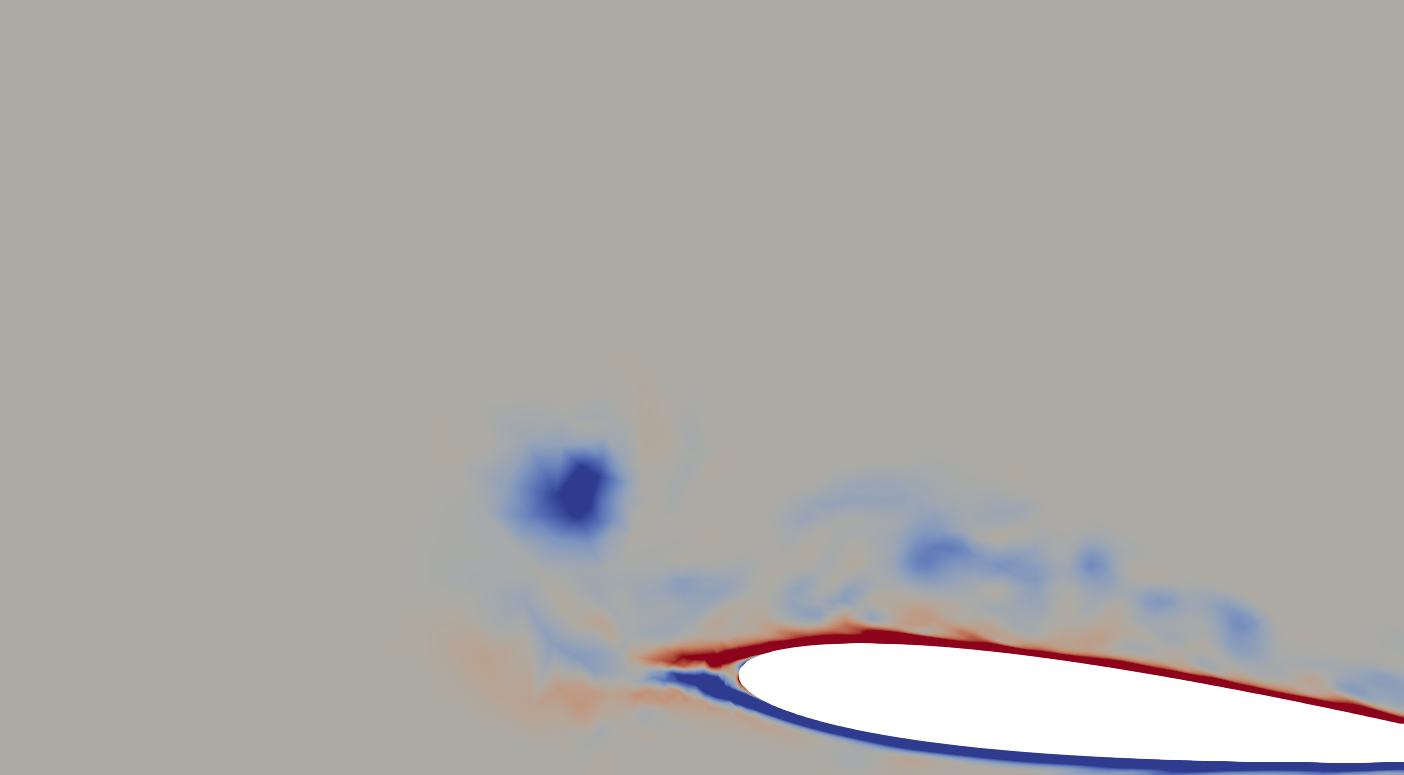
\includegraphics[width=1\textwidth]{figures/zonal_adapt_results/vorticity_plots/v3/M0/spavg/phase_270.png}
		\caption{M0\_nz25 mesh, $\psi$ = $270^\circ$}
		\label{fig:M0_sp_psi270}
		\end{subfigure}
	\end{center}
	\begin{subfigure}[b]{0.475\textwidth}
	\centering
	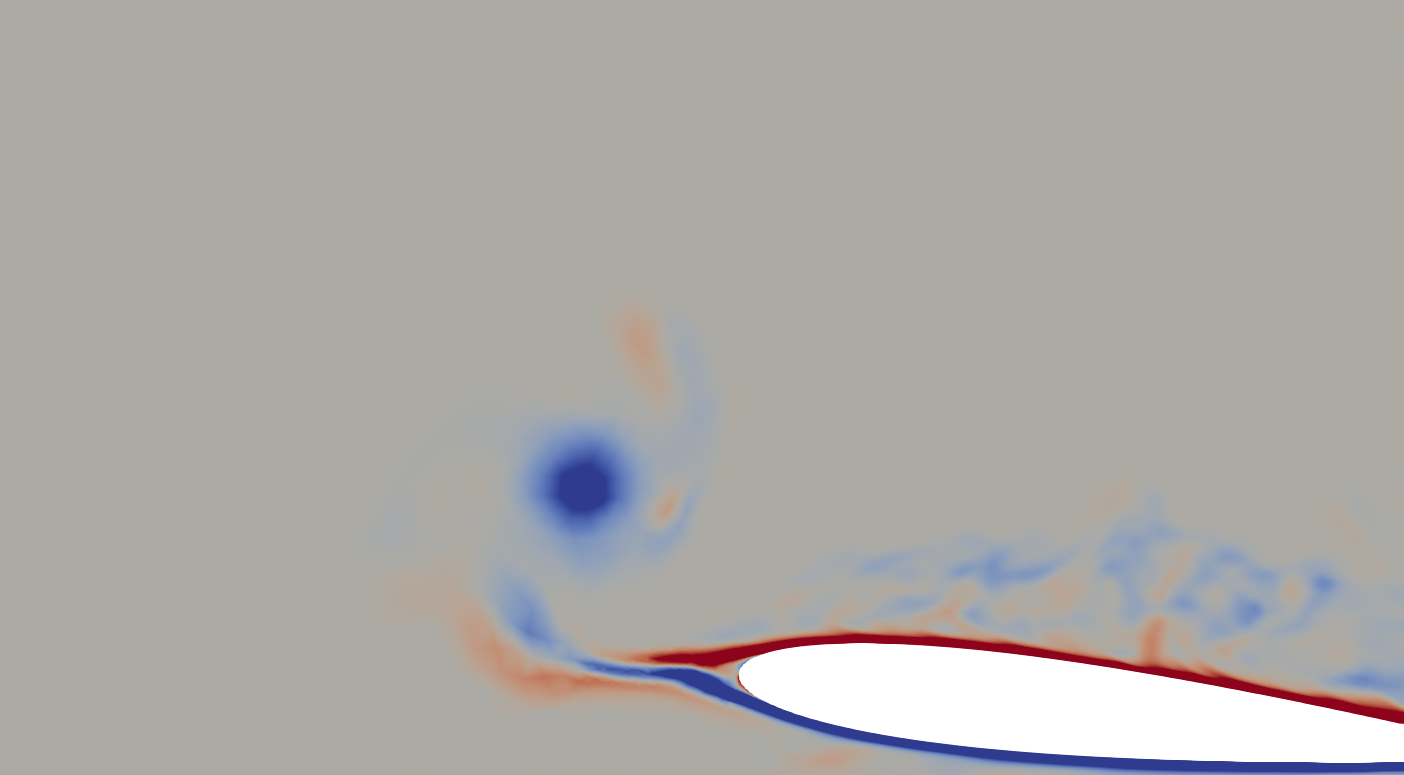
\includegraphics[width=1\textwidth]{figures/zonal_adapt_results/vorticity_plots/v3/Mza1_25/spavg/phase_270.png}
	\caption{Mza1\_nz25 mesh, $\psi$ = $270^\circ$}
	\label{fig:Mza1_25_sp_psi270}
	\end{subfigure}
	\begin{subfigure}[b]{0.475\textwidth}
		\centering
		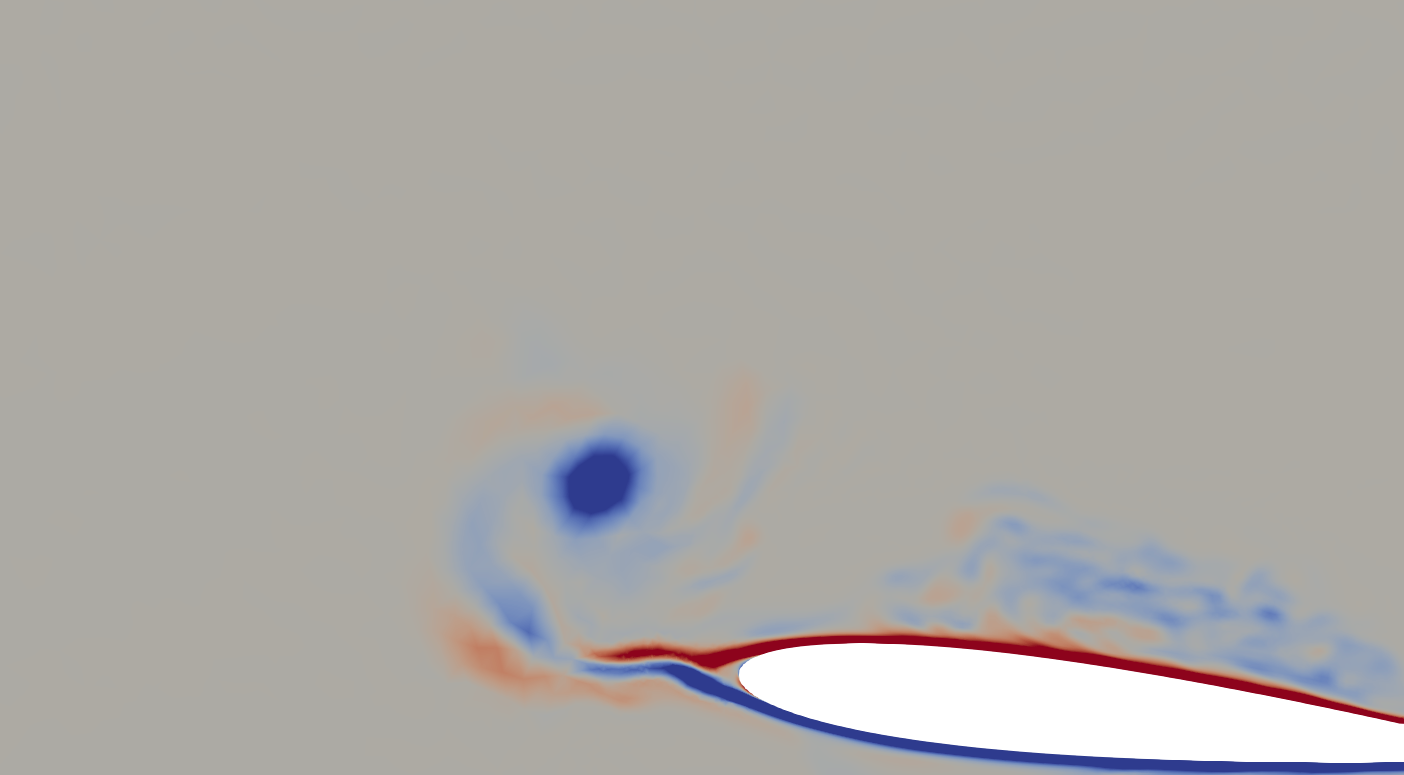
\includegraphics[width=1\textwidth]{figures/zonal_adapt_results/vorticity_plots/v3/Mza1_50/spavg/phase_270.png}
		\caption{Mza1\_nz50 mesh, $\psi$ = $270^\circ$}
		\label{fig:Mza1_50_sp_psi270}
	\end{subfigure}
%	\begin{subfigure}[b]{0.475\textwidth}
%		\centering
%		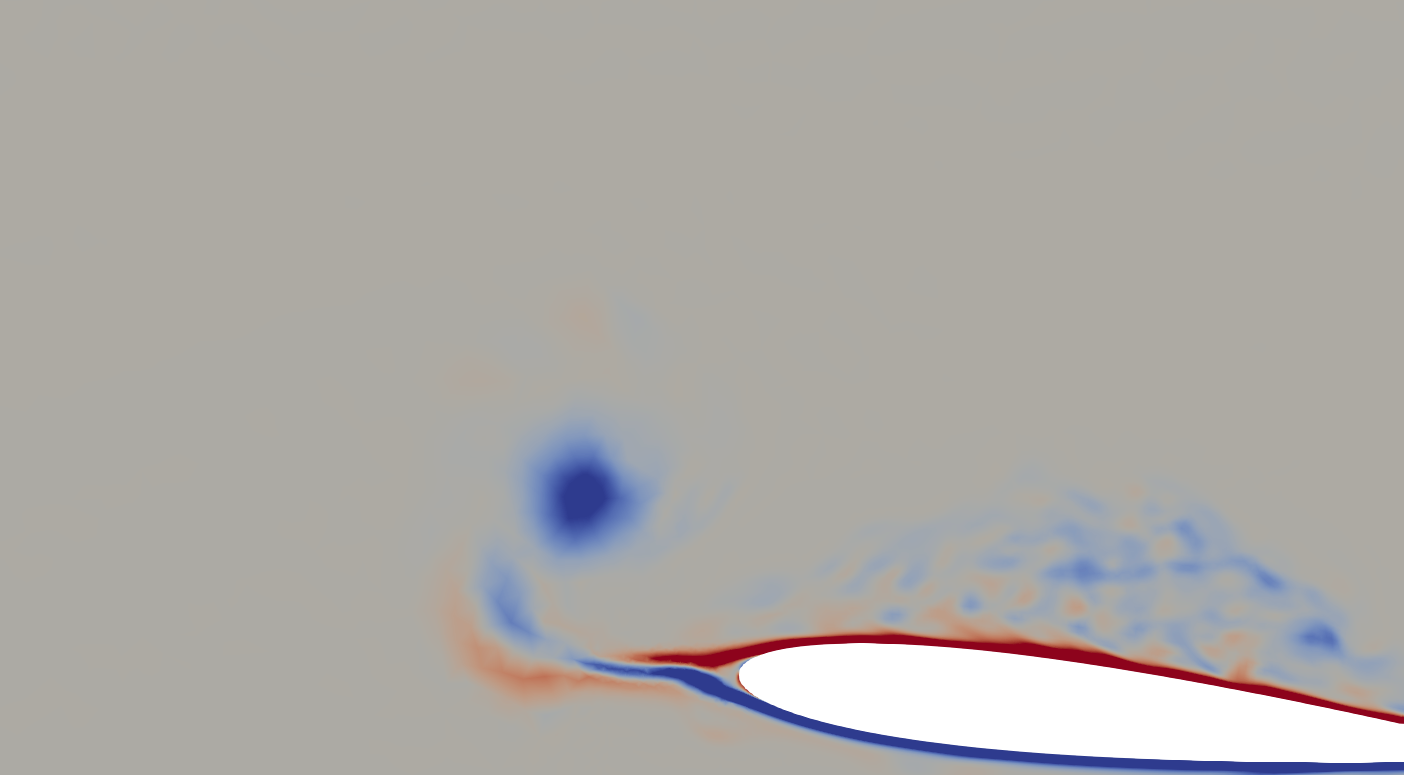
\includegraphics[width=1\textwidth]{figures/zonal_adapt_results/vorticity_plots/v3/Mza1_100/spavg/phase_270.png}
%		\caption{Mza1\_100 mesh, $\psi$ = $270^\circ$}
%		\label{fig:Mza1_100_sp_psi270}
%	\end{subfigure}
%	\begin{subfigure}[b]{0.475\textwidth}
%	\centering
%	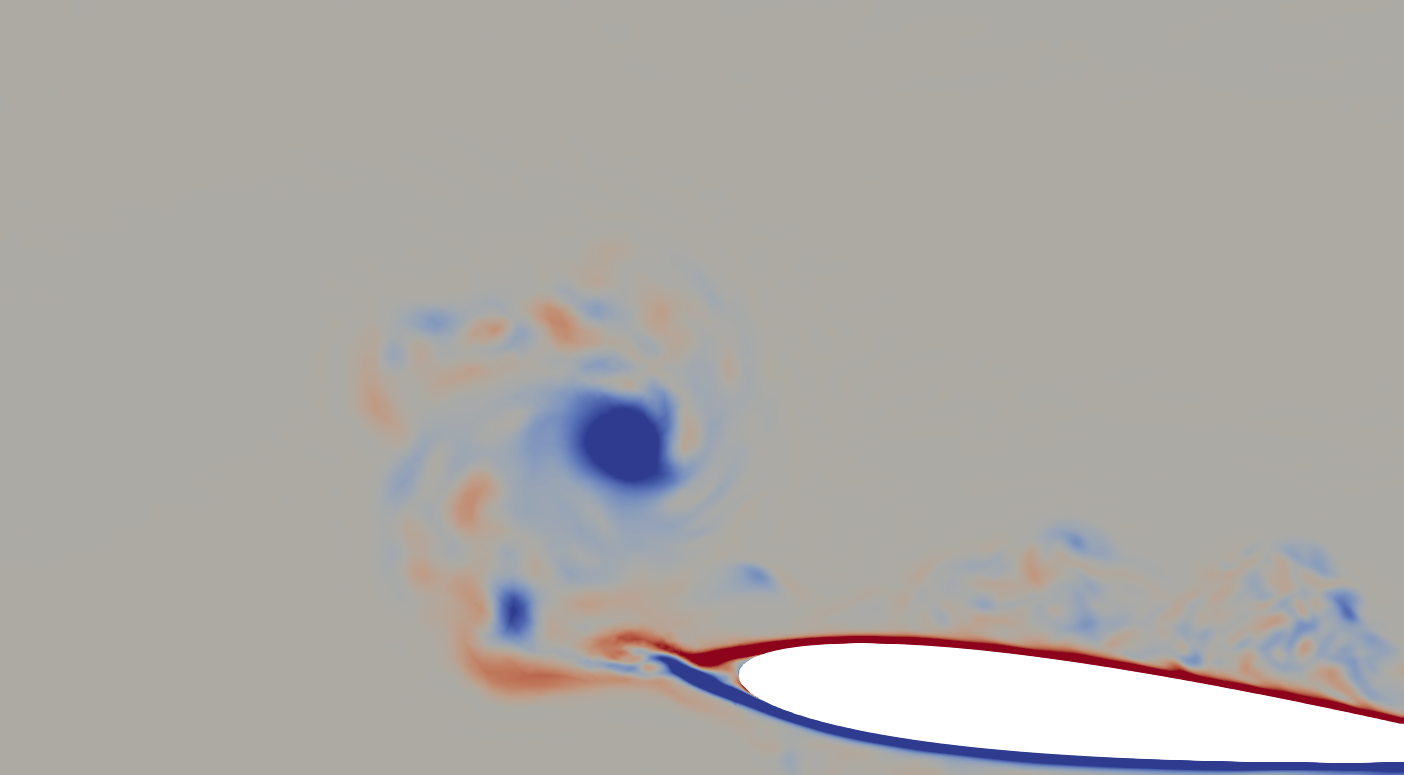
\includegraphics[width=1\textwidth]{figures/zonal_adapt_results/vorticity_plots/v3/Mza2_25/spavg/phase_270.png}
%	\caption{Mza2\_25 mesh, $\psi$ = $270^\circ$}
%	\label{fig:Mza2_25_sp_psi270}
%    \end{subfigure}	
	\begin{subfigure}[b]{0.475\textwidth}
		\centering
		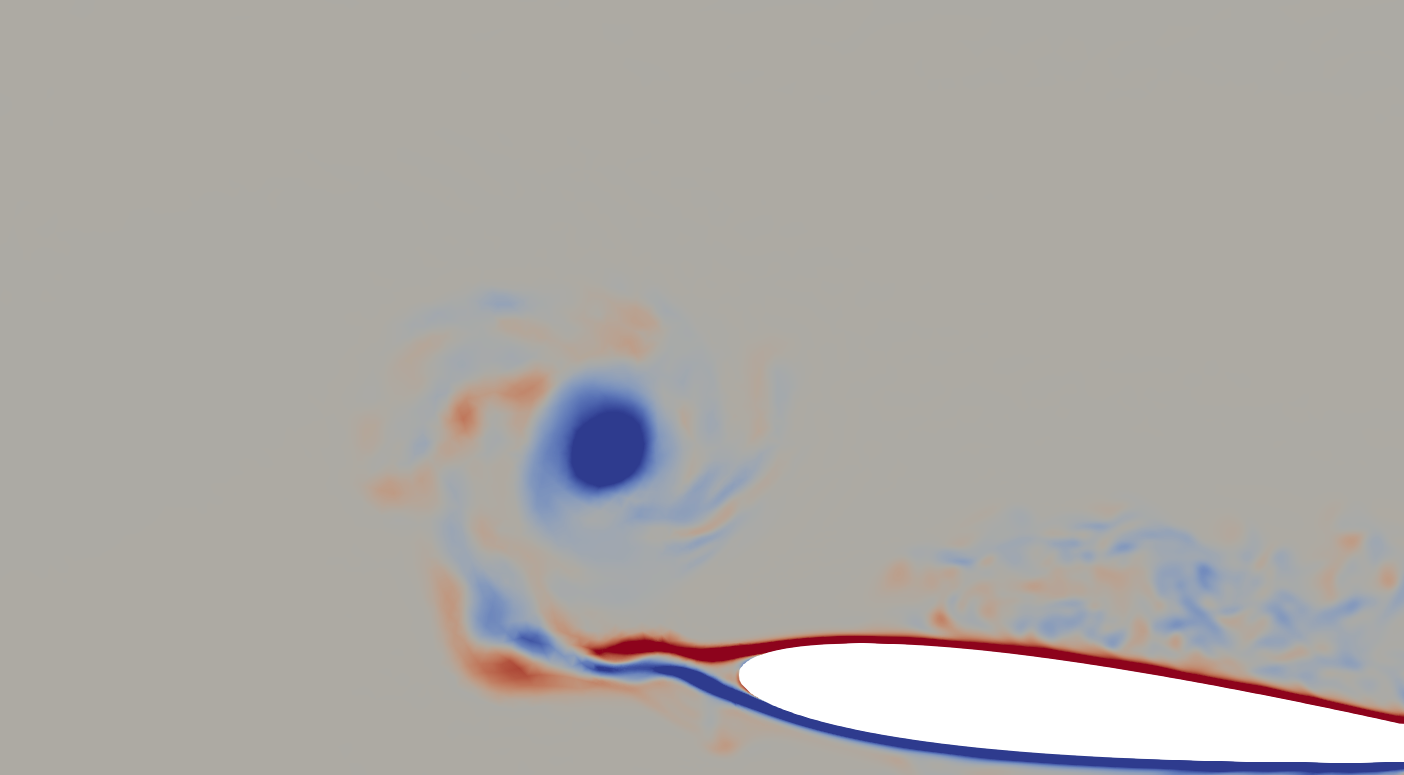
\includegraphics[width=1\textwidth]{figures/zonal_adapt_results/vorticity_plots/v3/Mza2_50/spavg/phase_270.png}
		\caption{Mza2\_nz50 mesh, $\psi$ = $270^\circ$}
		\label{fig:Mza2_50_sp_psi270}
	\end{subfigure}	
	\begin{subfigure}[b]{0.475\textwidth}
		\centering
		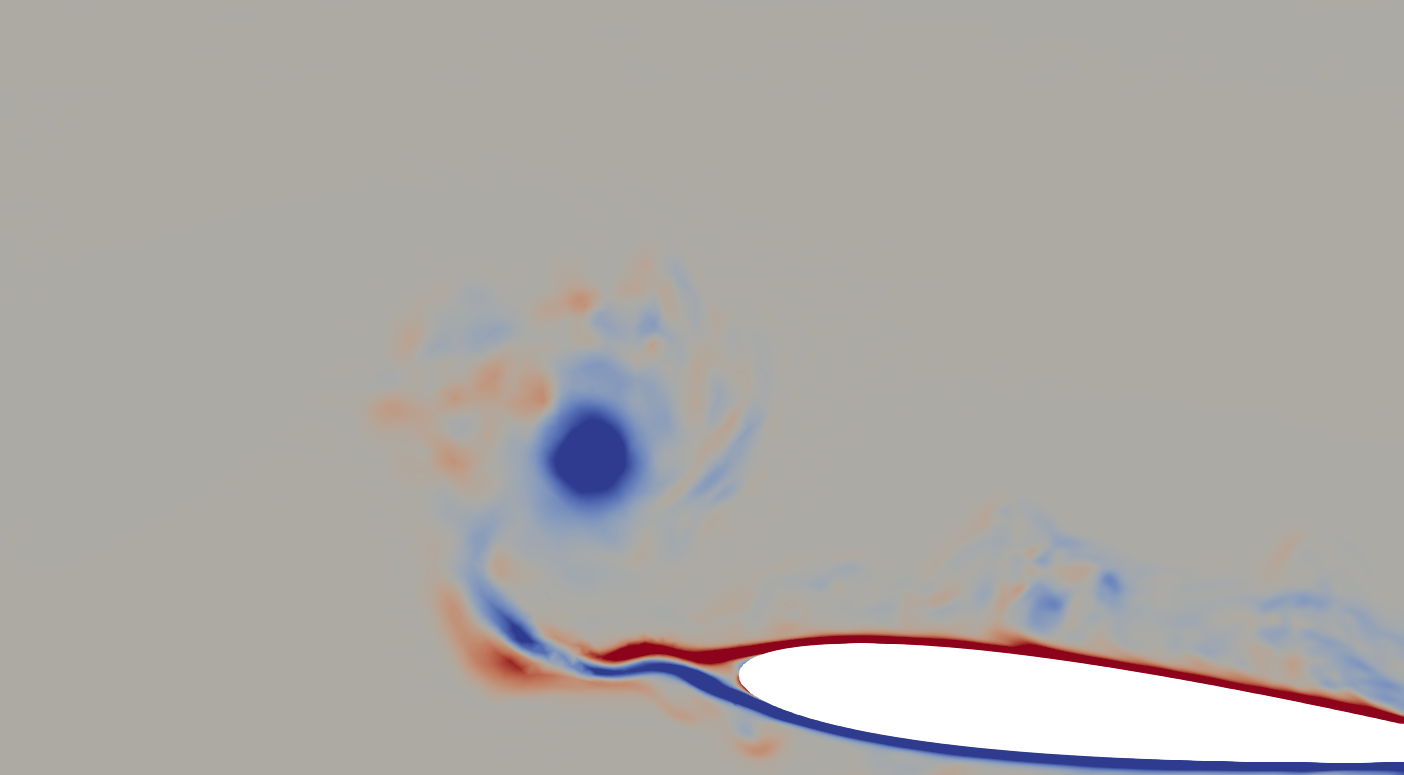
\includegraphics[width=1\textwidth]{figures/zonal_adapt_results/vorticity_plots/v3/Mza2_100/spavg/phase_270.png}
		\caption{Mza2\_nz100 mesh, $\psi$ = $270^\circ$}
		\label{fig:Mza2_100_sp_psi270}
	\end{subfigure}
	\begin{subfigure}[b]{0.475\textwidth}
	\centering
	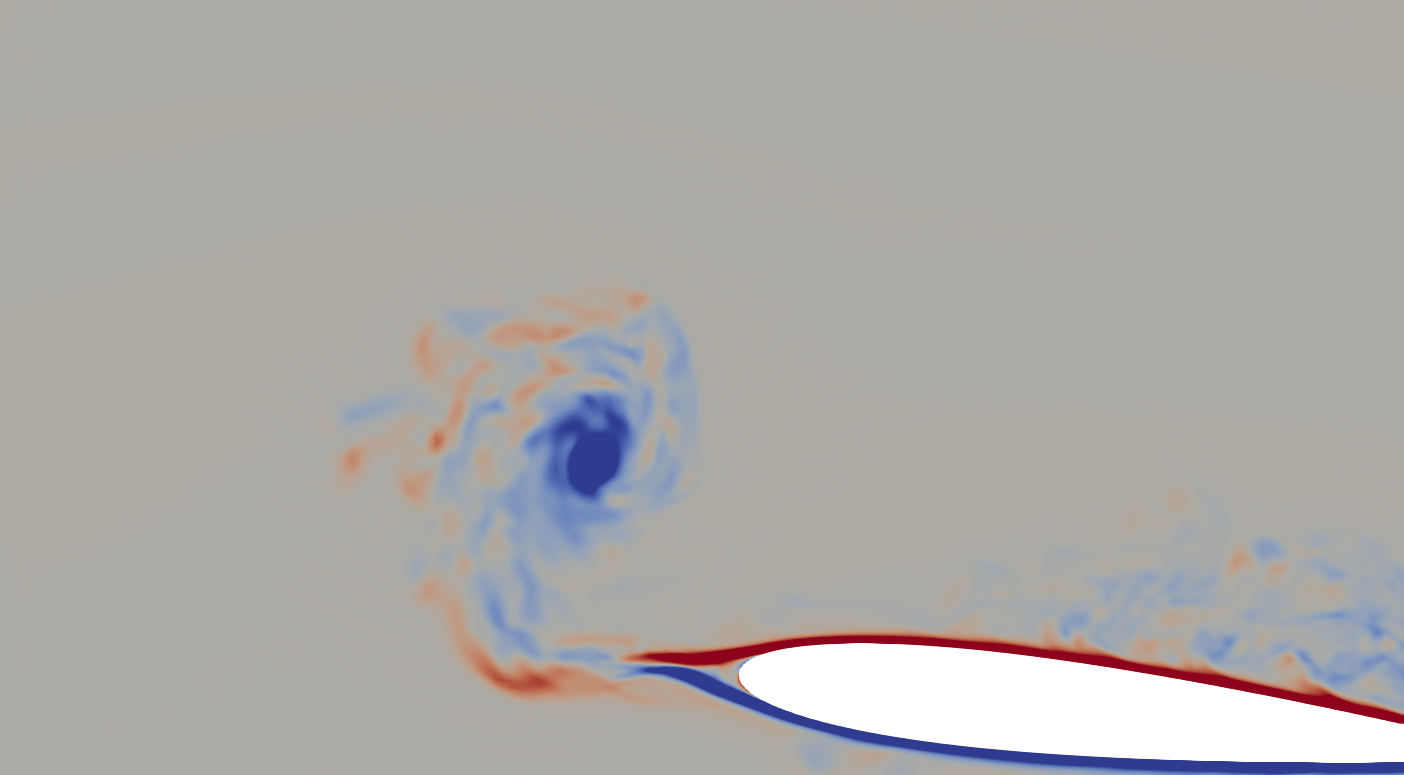
\includegraphics[width=1\textwidth]{figures/zonal_adapt_results/vorticity_plots/v3/Mza3_50/spavg/phase_270.png}
	\caption{Mza3\_nz50 mesh, $\psi$ = $270^\circ$}
	\label{fig:Mza3_50_sp_psi270}
\end{subfigure}
	\begin{subfigure}[b]{0.475\textwidth}
		\centering
		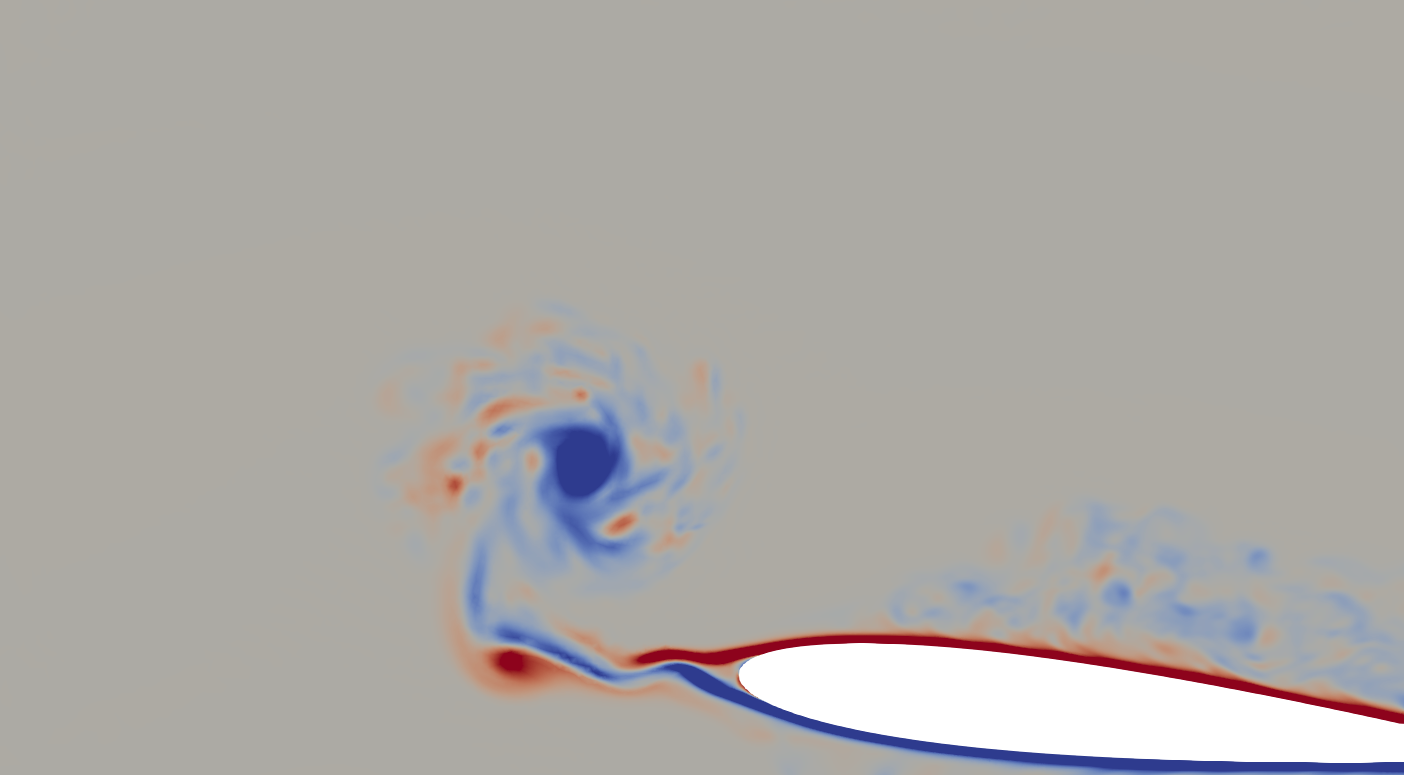
\includegraphics[width=1\textwidth]{figures/zonal_adapt_results/vorticity_plots/v3/Mza3_100/spavg/phase_270.png}
		\caption{Mza3\_nz100 mesh, $\psi$ = $270^\circ$}
		\label{fig:Mza3_100_sp_psi270}
	\end{subfigure}
	\caption{Spanwise vorticity comparison at $\psi$ = $270^\circ$ for different meshes}
	\label{fig:vorticity_zonal_270}
\end{figure}